%%%%%%%%%%%%%%%%%%%%%%%%%%%%%%%%%%%%%%%%%%%%
%Set Document Type
%%%%%%%%%%%%%%%%%%%%%%%%%%%%%%%%%%%%%%%%%%%%
\documentclass[11pt, a4paper]{report}  %Remove "twoside" for pdf version, keep for printing. 

%%%%%%%%%%%%%%%%%%%%%%%%%%%%%%%%%%%%%%%%%%%%
%Packages
%%%%%%%%%%%%%%%%%%%%%%%%%%%%%%%%%%%%%%%%%%%%
%\usepackage{MyStyle}
\usepackage{graphicx}
\usepackage{xspace}
\usepackage[svgnames]{xcolor}
\usepackage{longtable}
\usepackage{amsmath}     %!  setspace is used to control linepacing
%\usepackage[square]{natbib} %! needed for Harvard style of references.
\usepackage{enumerate}  %! used for the library form, but you might find 
\usepackage{hyperref}
\hypersetup{
    colorlinks=true,
    linkcolor=blue,
    citecolor=blue,
    filecolor=magenta,
    urlcolor=blue}
\usepackage[a4paper,width=150mm,top=30mm,bottom=25mm]{geometry} %Remove "left=4cm" for pdf version, keep for printing. 
\usepackage{multicol}
\usepackage{amssymb}
\usepackage{acro}
\usepackage{textgreek}
\usepackage{afterpage}
%%%%%%%%%%%%%%%%%%%%%%%%%%%%%%%%%%%%%%%%%%%%
%References
%%%%%%%%%%%%%%%%%%%%%%%%%%%%%%%%%%%%%%%%%%%%
\usepackage[backend=bibtex, style=authoryear]{biblatex}
\addbibresource{NewTools.bib} %Import the bibliography file
%%%%%%%%%%%%%%%%%%%%%%%%%%%%%%%%%%%%%%%%%%%%
%Set Tables
%%%%%%%%%%%%%%%%%%%%%%%%%%%%%%%%%%%%%%%%%%%%
\usepackage{lscape}
\usepackage{tablefootnote}
\usepackage{array}
\usepackage{bigfoot}
\usepackage{booktabs}
\usepackage{threeparttable}
\usepackage{multirow} 
% Add this line for caption customization
%%%%%%%%%%%%%%%%%%%%%%%%%%%%%%%%%%%%%%%%%%%%
%Set Font
%%%%%%%%%%%%%%%%%%%%%%%%%%%%%%%%%%%%%%%%%%%%
\usepackage[onehalfspacing]{setspace}
\usepackage[T1]{fontenc}
\usepackage{newpxtext,newpxmath}
%Set section headers to not be bold
\usepackage[titles]{tocloft, calc}
\renewcommand{\cftsecfont}{\mdseries}
\renewcommand{\cftsecpagefont}{\mdseries}
%%%%%%%%%%%%%%%%%%%%%%%%%%%%%%%%%%%%%%%%%%%%
%Set Figure and Table Caption colour
%%%%%%%%%%%%%%%%%%%%%%%%%%%%%%%%%%%%%%%%%%%%
\usepackage{caption}
\usepackage{subcaption} 
\captionsetup[table]{labelsep=period, labelfont={bf}, font={small, stretch=1.5}}     %% change 1.2 as you like
\captionsetup[figure]{labelsep=period, labelfont={bf}, font={small, stretch=1.5}}
\captionsetup{width=0.98\textwidth}
%%%%%%%%%%%%%%%%%%%%%%%%%%%%%%%%%%%%%%%%%%%%
%Set Code Block Formatting
%%%%%%%%%%%%%%%%%%%%%%%%%%%%%%%%%%%%%%%%%%%%
\usepackage{listings}
\usepackage{color}
%%%%%%%%%%%%%%%%%%%%%%%%%%%%%%%%%%%%%%%%%%%
%Chapter Style
%%%%%%%%%%%%%%%%%%%%%%%%%%%%%%
\usepackage{epigraph} %To add quotes
\usepackage{titlesec}
\usepackage{ulem}

\makeatletter
\def\@makechapterhead#1{%
    \vspace*{2em}% Space above number
    {\parindent \z@  \normalfont
    \interlinepenalty\@M
    \huge\centering{\scshape Chapter\ \thechapter}%
    \par\vspace{-2.63em}%
    \par\rule{.33\textwidth}{0.6pt}
    \par\vspace{0em}% Space between number and title
    \singlespacing\textbf{#1}%
    \par\vspace{2em}% Space between title and text
}}
\makeatother

\titleformat*{\section}{\Large\bfseries}
\titleformat*{\subsection}{\large\bfseries}
\titleformat*{\subsubsection}{\normalfont\bfseries}

%Paragraph Style
%%%%%%%%%%%%%%%%%%%%%%%%%%%%%%
\onehalfspacing
\usepackage{blindtext}
\usepackage{lastpage}
\usepackage{fancyhdr}
\usepackage{parskip}
\setlength{\parindent}{3em}

%Header and Footer Style
%%%%%%%%%%%%%%%%%%%%%%%%%%%%%%
\usepackage{xcolor}
\definecolor{headergray}{RGB}{128,128,128} % Define the grey color
\renewcommand{\headrule}{\textcolor{headergray}{\rule{\headwidth}{0pt}}} % Change the color of the header rule
\pagestyle{fancy}
\renewcommand{\sectionmark}[1]{\markboth{#1}{}}
\fancyhf{}
%\fancyhead[L]{\textcolor{headergray}{\small New Tools Thesis - Draft 1}}
\fancyhead[R]{\textcolor{headergray}{\small\chaptername~\thechapter | \leftmark}}
\fancyfoot{}
\fancyfoot[C]{\thepage}
%Prevent footnotes from breaking over multiple pages. 
\interfootnotelinepenalty=10000

%%%%%%%%%%%%%%%%%%%%%%%%%%%%%%%%%%%%%%%%                             
%Contents page
%%%%%%%%%%%%%%%%%%%%%%%%%%%%%%%%%%%%%%%%
\renewcommand{\cftchappresnum}{Chapter }
\AtBeginDocument{\addtolength\cftchapnumwidth{\widthof{\bfseries Chapter }}}

%%%%%%%%%%%%%%%%%%%%%%%%%%%%%%%%%%%%%%%%                             
%Acronyms
%%%%%%%%%%%%%%%%%%%%%%%%%%%%%%%%%%%%%%%%
                            
%Organism Names
%%%%%%%%%%%%%%%%%%%%%%%%%%%%%%%%%%%%%%%%
\DeclareAcronym{Focub}{
  short = \textit{Foc},
  long  = \textit{Fusarium oxysporum} f. sp. \textit{cubense}}

\DeclareAcronym{tr4}{
  short = TR4,
  long  = Tropical Race 4,
}

\DeclareAcronym{Focub4}{
  short = \textit{Foc} TR4,
  long  = \textit{Fusarium oxysporum} f. sp. \textit{cubense} Tropical Race 4}


\DeclareAcronym{str4}{
  short = STR4,
  long  = Sub-Tropical Race 4,
}

\DeclareAcronym{r1}{
  short = R1,
  long  = Race 1,
}
\DeclareAcronym{r4}{
  short = R4,
  long  = Race 4,
}

\DeclareAcronym{Focub1}{
  short = \textit{Foc} R1,
  long  = \textit{Fusarium oxysporum} f. sp. \textit{cubense} Race 1,
}
\DeclareAcronym{r2}{
  short = R2,
  long  = Race 2,
}  
  
\DeclareAcronym{Fo}{
  short = \textit{Fo},
  long  = \textit{Fusarium oxysporum},
}

\DeclareAcronym{Fs}{
  short = \textit{Fs},
  long  = \textit{Fusarium sacchari},
}

\DeclareAcronym{Ff}{
  short = \textit{Ff},
  long  = \textit{Fusarium fujikuroi},
}

\DeclareAcronym{Fol}{
  short = \textit{Fol},
  long  = \textit{Fusarium oxysporum} f. sp. \textit{lycopersici},
}

\DeclareAcronym{Fon}{
  short = \textit{Fon},
  long  = \textit{Fusarium oxysporum} f. sp. \textit{niveum},
}


\DeclareAcronym{fsp}{
  short = f. spp.,
  long  = \textit{Formae speciales},
}

\DeclareAcronym{FFSC}{
  short = FFSC,
  long  = \textit{Fusarium fujikuroi} species complex,
}  

\DeclareAcronym{FOSC}{
  short = FOSC,
  long  = \textit{Fusarium oxysporum} species complex,
} 

\DeclareAcronym{FGSC}{
  short = FGSC,
  long  = \textit{Fusarium graminearum} species complex,
} 

\DeclareAcronym{vcg}{
  short = VCG,
  long  = Vegetative Compatibility Group,
} 

\DeclareAcronym{xvm}{
  short = \textit{Xvm},
  long  = \textit{Xanthomonas   campestris }pv. \textit{musacearum},
} 

\DeclareAcronym{fwb}{
  short = FWB,
  long  = \textit{Fusarium} wilt of banana} 

%Genes, Proteins etc
%%%%%%%%%%%%%%%%%%%%%%%%%%%%%%%%%%%%%%%%
\DeclareAcronym{tef}{
  short = \textit{Tef-1}\textalpha,
  long  = \textit{Translation Elongation Factor-1} \textalpha ,
}

\DeclareAcronym{rbp2}{
  short = \textit{RPBii},
  long  = \textit{RNA polymerase   subunit 2},
}

\DeclareAcronym{mites}{
  short = MITEs,
  long  = Miniature inverted-repeat transposable elements,
}

\DeclareAcronym{te}{
  short = TE,
  long  = transposable element,
}

\DeclareAcronym{mimp}{
  short = \textit{mimp},
  long  = \textit{\underline{m}iniature \underline{imp}ala},
}

\DeclareAcronym{sixg}{
  short = \textit{SIX} gene,
  long  = \textit{Secreted In Xylem  } gene,
}

\DeclareAcronym{sixp}{
  short = SIX protein,
  long  = Secreted In Xylem protein,
}

\DeclareAcronym{vic}{
  short = \textit{Vic},
  long  = \textit{Vegetative Incompatibility}}

\DeclareAcronym{rga2}{
  short = \textit{RGA2},
  long  = \textit{Resistance Gene Analog 2}}



%Biologial Processes & General Terms
%%%%%%%%%%%%%%%%%%%%%%%%%%%%%%%%%%%%%%%%
\DeclareAcronym{AVR}{
short = AVR,
long = avirulence,
}

\DeclareAcronym{ac}{
short = AC,
long = accessory chromosome,
}

\DeclareAcronym{cc}{
short = CC,
long = core chromosome,
}

\DeclareAcronym{bp}{
short = bp,
long = base pair,
}

\DeclareAcronym{tir}{
short = TIR,
long = Terminal Invert Repeat,
}

\DeclareAcronym{prr}{
short = PRRs,
long = pattern recognition receptors,
}

\DeclareAcronym{nlr}{
short = NLR,
long = nucleotide-binding leucine-rich receptor,
}

\DeclareAcronym{pamp}{
short = PAMPs,
long = pathogen-associated molecular patterns,
}

\DeclareAcronym{pti}{
short = PTI,
long = PAMP-triggered immunity,
}


\DeclareAcronym{pcr}{
short = PCR,
long = polymerase chain reaction,
}
  
\DeclareAcronym{eti}{
short = ETI,
long = effector-triggered immunity,
}

\DeclareAcronym{ets}{
short = ETS,
long = effector-triggered susceptibility,
}

\DeclareAcronym{rprot}{
short = R proteins,
long = resistance proteins,
}

\DeclareAcronym{rgene}{
short = R gene,
long = resistance gene,
}

                         
%Bioinf 
%%%%%%%%%%%%%%%%%%%%%%%%%%%%%%%%%%%%%%%%
\DeclareAcronym{blast}{
short = BLAST,
long = Basic Local Alignment Tool,
}

\DeclareAcronym{busco}{
short = BUSCO,
long = Benchmarking Universal Single-Copy Orthologs,
}

\DeclareAcronym{maei}{
short = Maei,
long = \textit{Mimp}-associated effector identification,
}

\DeclareAcronym{ml}{
short = ML,
long = Machine learning,
}

\DeclareAcronym{phibase}{
short = PHI-base,
long = Pathogen-Host Interaction Database,
}               

%Stats
%%%%%%%%%%%%%%%%%%%%%%%%%%%%%%%%%%%%%%%%
\DeclareAcronym{ANOVA}{
short = ANOVA,
long = Analysis of variance,
}

\DeclareAcronym{hmm}{
short = HMM,
long = Hidden Markov Model}

%Experimental Terms and Techniques
%%%%%%%%%%%%%%%%%%%%%%%%%%%%%%%%%%%%%%%%

\DeclareAcronym{dpi}{
short = dpi,
long = Days post-inoculation,
}

\DeclareAcronym{wpi}{
short = wpi,
long = Weeks post-inoculation,
}

\DeclareAcronym{hplc}{
short = HPLC,
long = High-performance liquid chromatography,
}

\DeclareAcronym{lcms}{
short = LCMS,
long = Liquid Chromatography-Mass Spectrometry,
}

\DeclareAcronym{lamp}{
short = LAMP,
long = Loop-mediated isothermal amplification
}

\DeclareAcronym{pda}{
short = PDA,
long = Potato dextrose agar,
}

\DeclareAcronym{pdb}{
short = PDB,
long = Potato dextrose broth,
}

\DeclareAcronym{rpm}{
short = rpm,
long = Revolutions per minute
}

\DeclareAcronym{um}{
short = UM,
long = untargeted metabolomics,
}

%Organisations
%%%%%%%%%%%%%%%%%%%%%%%%%%%%%%%%%%%%%%%%
\DeclareAcronym{FAO}{
short = FAO,
long = Food and Agriculture Organisation of the United Nations}

\DeclareAcronym{wbf}{
short = WBF,
long = World Banana Forum}

\DeclareAcronym{ncbi}{
short = NCBI,
long = National Center of Biotechnology Information, }

\DeclareAcronym{tnau}{
short = TNAU,
long = Tamil Nadu Agricultural University }

%Misc
%%%%%%%%%%%%%%%%%%%%%%%%%%%%%%%%%%%%%%%%

\DeclareAcronym{rs}{
short = RS,
long = remote sensing }

\DeclareAcronym{uav}{
short = UAV,
long = Unmanned Aerial Vehicle}

\DeclareAcronym{vi}{
short = VI,
long = Vegetation Indices}

\DeclareAcronym{ps2}{
short = PSII,
long = Photosystem II}

\newcommand{\et}{\textit{et al., }}


%%%%%%%%%%%%%%%%%%%%%%%%%%%%%%%%%%%%%%%%                             
%Start Document
%%%%%%%%%%%%%%%%%%%%%%%%%%%%%%%%%%%%%%%%
\linespread{2} 
\begin{document}

%%%%%%%%%%%%%%%%%%%%%%%%%%%%%%%%%%%%%%%%
%Title Pages
%%%%%%%%%%%%%%%%%%%%%%%%%%%%%%%%%%%%%%%%
\begin{titlepage}
\begin{titlepage}
    \begin{center}
        \singlespacing
        \Huge
        \textbf{New Tools for the Identification of} \\\vspace*{0.5cm} \textbf{\textit{Fusarium} Wilt in Banana} \\
        \vspace*{1.75cm}
        \normalsize
        by \\ 
        \vspace*{0.2cm}
        \LARGE
        Jamie Pike BSc (Hons) \\ 
        \vfill
        \normalsize
        Submitted in the partial fulfilment of the requirements for the degree of \\
        \Large
        \vspace*{0.3cm}
        Doctor of Philosophy in Life Sciences \\
        \vspace*{1cm}
        \includegraphics[width=0.4\textwidth]{Preamble/crest_black.eps} \\
        \vspace*{1cm}
        \large
        University of Warwick, School of Life Sciences\\
        \vspace*{0.5cm}
        \normalsize
        March 2024 \\
         \vspace*{1cm}   
    \end{center}
    \clearpage
\end{titlepage}
\end{titlepage}
\newpage
\thispagestyle{empty} 
%%%%%%%%%%%%%%%%%%%%%%%%%%%%%%%%%%%%%%%%
%Fromatting
%%%%%%%%%%%%%%%%%%%%%%%%%%%%%%%%%%%%%%%%
\pagenumbering{roman} %! Begins roman numerals start from page i.

%%%%%%%%%%%%%%%%%%%%%%%%%%%%%%%%%%%%%%%%
%Table of Contents
%%%%%%%%%%%%%%%%%%%%%%%%%%%%%%%%%%%%%%%%
\clearpage
\tableofcontents
\listoftables                     
\listoffigures  

\addtocontents{toc}{\protect\setlength{\cftbeforechapskip}{0pt}}
%%%%%%%%%%%%%%%%%%%%%%%%%%%%%%%%%%%%%%%%
%Prelimary Sections
%%%%%%%%%%%%%%%%%%%%%%%%%%%%%%%%%%%%%%%%

\setcounter{secnumdepth}{-2}% default for "report" is 2

% \cleardoublepage
% \phantomsection
% \addcontentsline{toc}{chapter}{Acknowledgements}
% \chapter*{\huge\centering Acknowledgements}

% \cleardoublepage
% \phantomsection
% \addcontentsline{toc}{chapter}{Thesis Declaration}
% \chapter*{\huge\centering Thesis Declaration}

% \cleardoublepage
% \phantomsection
% \addcontentsline{toc}{chapter}{Inclusion of Published Work}
% \chapter*{\huge\centering Inclusion of Published Work}

% \cleardoublepage
% \phantomsection
% \addcontentsline{toc}{chapter}{Abstract}
% \chapter*{\huge\centering Abstract}

\cleardoublepage
\phantomsection
\addcontentsline{toc}{chapter}{Abbreviations}
\chapter*{\huge\centering Abbreviations}  
\printacronyms[heading=none]

\clearpage

\setcounter{secnumdepth}{2}

      
%%%%%%%%%%%%%%%%%%%%%%%%%%%%%%%%%%%%%%%%%%%%
%Main Chapters
%%%%%%%%%%%%%%%%%%%%%%%%%%%%%%%%%%%%%%%%
\pagenumbering{arabic} %! Begins arabic numerals start from page 1.
\renewcommand{\arraystretch}{1.5} %Extend tables so they're easier to read
%Set all instances of text below (e.g. \focub) to italicised full version.

% %Set chapter names and .tex files with chapter content.
% \setlength\epigraphwidth{.7\textwidth}
% \setlength{\epigraphrule}{0pt}
    
\chapter{General Introduction}\label{Chap1}
    \section {An Introduction to Banana}

Banana (\textit{Musa} spp.) is frequently reported as one of the world’s top agricultural commodities. Annual global production of bananas (including plantain) steadily increased from 98.4 million tonnes in 2000 to an estimated 155.2 million tonnes in 2018 (\ac{FAO}, 2020). A staple food and cash crop of significant agricultural, financial, and social importance, only around 15\% of bananas produced worldwide are traded in international markets, the remaining 85\% are consumed locally (\ac{FAO}, 2018), highlighting the value of bananas as a subsistence crop. Particularly in developing countries where fruits can account for 25\% of daily calorie intake and act as a source of income (\ac{FAO}, 2018).

\subsection{Anatomy and Classification of Banana}  

Banana is a monocotyledonous, herbaceous perennial which belongs to the Musaceae family in the order Zingiberales (Table ~\ref{tab:TaxonTable}) (Schoch \et 2020). Currently, there are 74 species of \textit{Musa} accepted by the World Checklist of Selected Plant Families (WCSP, 2022), including wild, ornamental, and cultivated species. Linnaeus originally described two species of banana: \textit{M. sapientum }and \textit{M. paradisiaca}. However, the classification of banana using the formalised binomial system following Linnaeus proved ineffective due to banana’s complicated genetic history (Cheesman, 1947).  

% Please add the following required packages to your document preamble:
% \usepackage{longtable}
% Note: It may be necessary to compile the document several times to get a multi-page table to line up properly
\begingroup
\setlength{\tabcolsep}{15pt} % Default value: 6pt
\renewcommand{\arraystretch}{0.9}
\begin{longtable}[c]{cc}
\caption[Taxonomy of \textit{Musa} genus]{\textbf{Taxonomy of \textit{Musa} genus including 3 example species} (Schoch et al., 2020, WCSP, 2022).}
\label{tab:TaxonTable}\\
\hline
\textbf{Kingdom}     & Plantae       
\endfirsthead
%
\multicolumn{2}{c}%
{{\bfseries Table \thetable\ continued from previous page}} \\
\endhead
%
\textbf{Phylum}      & Tracheophytes \\ 
\textbf{Class}       & Magnoliopsida \\ 
\textbf{Super order} & Lilianae      \\ 
\textbf{Order}       & Zingiberales  \\ 
\textbf{Family}      & Musaceae      \\ 
\textbf{Genus}       & \textit{Musa} \\ 
\textbf{Species} & \textit{\begin{tabular}[c]{@{}c@{}}M. acuminata,\\
M. balbisiana, \\
M. basjoo\end{tabular}} \\ \hline
\end{longtable}
\endgroup

In the mid-20th century, Cheesman, (1947) recognised the two species described by Linnaeus to be cultivars of wild the \textit{Musa} species \textit{M. acuminata }and \textit{M. balbisiana} and regrouped the remaining \textit{Musa} species into 4 ‘sections’. Building on the work of Cheesman, Simmonds and Shepherd, (1955) developed a genome-based, informal nomenclature system for cultivated banana which is still used today. The system classifies varieties into genome groups based on the ploidy contribution of their wild ancestors, where the species contribution is denoted by the letters ‘A’ and ‘B’ for \textit{M. acuminata} and \textit{M. balbisiana}, respectively. For example, “Cavendish banana (\textit{Musa }spp. AAA group) cv. ‘Grand Nain’” indicates the variety’s sub-group (Cavendish), genus (\textit{Musa}), genome group scoring (AAA), and cultivar (Grand Nain).

The anatomy of banana plants is outlined in detail by Robinson and Saúco, (2010) and Bakry \et (2009). Briefly, plants produce a fibrous root system from a tuberous rhizome. Extended horizontal growth, typical of most rhizomatous plants, is not observed in banana; the plant instead produces suckers which successively grow outwards from the short rhizome. The leaves are produced from the central meristem of the rhizome, or developing sucker, and laminae continue to widen until they mature. As leaf sheaths develop, they become tightly packed and thicken to form the pseudostem which elongates as more leaves emerge to 1-8m in height (Bakry \et 2009) (Figure ~\ref{fig:Anatomy of fruiting banana plant}). 

\begin{figure}[hp]
    \centering
    \includegraphics[width=12cm]{Figures/Diagrammatic-representation-of-a-fruiting-banana-plant-with-suckers-in-Bakry-et-al_W640.jpg}
    \caption[Anatomy of fruiting banana plant]{\textbf{Anatomy of fruiting banana plant} (From Bakry, et al. (2009)).}
    \label{fig:Anatomy of fruiting banana plant}
\end{figure}

\subsection{The History, Cultivation, and Value of Banana}

Originating from Southeast Asia, naturally occurring parthenocarpic – development of fruit without fertilisation – individuals of banana have been cultivated for about 10,000 years. Evidence of this can been seen in \textit{Musa banksii} phytoliths discovered in the Kuk swamp in Papua New Guinea (Denham, 2011). Cultivated bananas were spread from Papua New Guinea, hybridising with other subspecies of \textit{M. acuminata} and \textit{M. balbisiana} in the Philippines and northern New Guinea (Perrier \et 2009). Triploid cultivars were produced as a consequence and were dispersed throughout Southeast Asia, Northern Australia, East Africa, and South Asia by the Austronesian peoples; where, although primarily cultivated as a food crop, banana was used in traditional medicine to treat ailments including dysentery, ulcers, leprosy, epilepsy and insect bites (Kumar \et 2012). In these regions, banana has also been used as fodder; in domestic materials, such as plates, children’s toys and dyes; in building for shelter, rafts, or rope; and has significant social and cultural value, involved in many traditional rituals and customs (Hapsari \et 2017).  

Banana cultivation continued to move into the Middle East and Northern Africa from the centre of domestication in Southeast Asia, which can be seen in references banana in Islamic texts such as Ibn al-'Awwam's 12th-century agricultural work, Book on Agriculture (Clément-Mullet, 1866). During expeditions in Southeast Asia and Africa in the mid-1500s, bananas were encountered by Europeans (Amano \et 2021) who transported plants to South America where colonists established banana plantations to supply the USA and Europe (Guzmán-Rivas, 1960, Salas-Pascual and Cáceres-Lorenzo, 2022). This legacy continues today, with over 70\% of the EU’s banana supply coming from South American countries (EuropeanUnion, 2022).  

Banana production takes place year-round in tropical and subtropical regions, where plants are commercially grown as a monoculture crop. Plants are also cultivated by smallholders and in subsistence production systems (Viljoen \et 2020). Commercially, fruits are harvested within about 9-12 months of planting (either\textit{ in vitro} propagated material or suckers) and are grown as a ratoon crop – the plant is cut back to the rhizome once the fruit has been harvested and left to regrow – for several years, by which time yields will have reduced and a new plantation must be generated (BananaLink, 2020). The world’s largest banana growers are India and China which produced over 30 million tonnes and 11 million tonnes in 2018, respectively.  Currently, up to 40\% of all global banana production (domestic and export markets) is reliant on the Cavendish bananas (Warman and Aitken, 2018), a triploid, clonally propagated subgroup deriving from \textit{M. acuminata}. 

\subsection{Bananageddon! \textit{\acl{Fo}} and Current Banana Production}

In recent decades, there have been increasing reports of a potential ‘Bananageddon!’, whereby global banana production is decimated by the soil-borne, fungal pathogen \acl{Focub} (\ac{tr4}), the causative agent of Fusarium wilt of banana (syn. Panama disease). The global banana community’s concern is reflected in the establishment of the \ac{tr4} Task Force as part of the \ac{FAO}'s \ac{wbf}, the Peruvian government’s decision to declare a National Emergency upon the discovery of \ac{Focub} \ac{tr4} in 2021 (FAO, 2021), and in the recent publication by van Westerhoven \et (2022), where the authors stress the threat \ac{Focub} poses to African food security.   

\section{An Introduction to \acl{Focub}}

\subsection{A Brief History of Fusarium Wilt}

The robust response to \ac{Focub4} s not unfounded. During the first half of the 20th century, \ac{Focub} \ac{r1} devastated global production until the resistant banana subgroup, Cavendish, was identified. \ac{Focub} \ac{r1} destroyed approximately 40,000 hectares of ‘Gros Michel’ plantations (Agrios, 2005), and resulted in estimated economic losses of \$400 million (USD) between 1940 and 1960 (Ploetz, 2005). \ac{Focub} \ac{r1} led to the disappearance of ‘Gros Michel’ as an export banana in the 1960s (Molina \et 2007).  

Cavendish bananas were identified as resistant to \ac{Focub} \ac{r1} and subsequently replaced ‘Gros Michel’ (Ordonez \et 2015). However, from the 1960s Cavendish banana plants in Taiwan were observed displaying symptoms of \ac{Focub} infection (Agrios, 2005). Identified in 1994 as \acl{Focub4} (Ploetz, 1994), the strain affecting Cavendish bananas has continued to spread. \ac{Focub4} is now found in Africa, Asia and Europe (Ploetz, 2015a, Thangavelu \et 2019) and is gaining a foothold in South America with recent incursions in Columbia in 2019 (Garcia-Bastidas \et 2019), Peru in 2021 (\ac{FAO}, 2021), and Venuzuela in 2023 (Herrera, \et 2023).

\subsection{Disease Development of \acl{Focub}}

As a soil-borne pathogen, \ac{Focub} first colonises the roots. Asexual spores found in the soil germinate in response to host root exudates. Infection hyphae produced from resting spores (chlamydospores) penetrate the root epidermis at the tip. \ac{Focub} hyphae progress through the root cortex to the rhizome. \ac{Focub} migrates through the xylem in the outer leaf sheaths of the pseudostem occluding vessels and interferes with nutrient uptake and upward water transport; often before external symptoms are observed (Li \et 2017a, Warman and Aitken, 2018). Two asexual spore types, microconidia and macroconidia, are produced within the xylem and help \ac{Focub} overcome some of the host’s barriers, such as naturally occurring end walls or perforation plates of the xylem strands which somewhat inhibit pathogen movement through the host (Dita \et 2018). Xylem vessels begin to collapse, and external symptoms are observed. Tissues become chlorotic and the plant withers as it transpires more than it can translocate. Once the plant dies, the fungus begins to invade other plant tissues and sporulate, particularly on the plant surface, producing chlamydospores (Figure ~\ref{fig:MyLifeCylce}). Chlamydospores can persist in the soil for decades and are resistant to adverse conditions (Pegg \et 2019).  

\begin{figure}[hp!]
    \centering
    \includegraphics[width=14cm]{Figures/MyLifeCylceNarrow.pdf}
    \caption[Fusarium wilt of banana disease cycle.]{\textbf{Fusarium wilt of banana disease cycle.} Chlamydospores germinate in the soil in response to plant root exudates. Infection hyphae from Chlamydospores penetrate the root tip epidermal cells and progress through then host root cortex to the xylem. Microconidia and macroconidia are produced in the xylem and help to facilitate pathogen movement through the host. As Foc migrates through the xylem it occludes vessels and interferes with nutrient uptake and upward water transport. External wilting symptoms begin to develop; tissues become chlorotic and the plant withers as it transpires more than it can translocate. Eventually, the plant dies, and asexual spores are formed on the dead tissue. Chlamydospores persist in the soil or Foc survives endophytically in an alternative host species. Fungal hyphae are shown in blue. Images of Foc spores adapted from Fourie \et  (2011) and symptomatic banana plant images sourced from Maymon \et  (2020). Figure created with BioRender.com.}
    \label{fig:MyLifeCylce.}
\end{figure}


Alternative hosts, including many grass and weed species, also act as a reservoir of inoculum (Hennessy \et 2005).  \ac{Focub} is dispersed through the movement of contaminated plant and soil material, water, wind, and people. Typical symptoms of \ac{Focub} infection include pseudostem splitting and discolouration, yellowing of lower leaves often forming a ‘skirt’ around the plant, and, occasionally, a streaking pattern is observed on the foliage (Figure ~\ref{fig:FusariumWiltSymptoms}). 

\begin{figure}[hpt!]
    \centering
    \includegraphics[width=15cm]{Figures/SymptomsofFoc.pdf}
    \caption[Typical symptoms of Fusarium  wilt of banana.]{\textbf{Typical symptoms of \textit{Fusarium} wilt of banana.} (a) Splitting of the psuedostem, (b) discolouration of the psuedostem, (c) yellowing of lower leaves, and (d), a streaking pattern is observed on the foliage.}
    \label{fig:FusariumWiltSymptoms}
\end{figure}

\subsection{Classification of \acl{Focub}}

\ac{Focub} belongs to the \ac{FOSC}. The species complex contains both plant and animal pathogens, as well as saprophytes and endophytes (Leslie and Summerell, 2006). \ac{Fo} has high functional and genetic diversity, shown plainly in its broad plant host range. The species complex can infect around 150 species of both monocotyledonous and dicotyledonous plants, including many horticulturally significant crops such as banana, tomato and lettuce  (Edel-Hermann and Lecomte, 2019).  Individual pathogenic \ac{Fo} isolates can infect only one or a few plant species. Plant pathogenic \ac{Fo} are therefore divided into ‘special forms’, or (\ac{fsp}), each of which is adapted to specific hosts (Snyder and Hansen, 1940). For instance, strains which cause Fusarium wilt in tomato are classified as \ac{Fol}. To date, 106 \ac{fsp} have been clearly described and with at least an additional 37 putative \ac{fsp} (Edel-Hermann and Lecomte, 2019).   

Some \ac{fsp} can be further subdivided into pathogenic races, determined by pathogenicity towards specific host cultivars. Three races of \ac{Focub} affecting banana have been identified. \acl{r1} affects banana cultivars such as ‘Gros Michel’ (AAA), ‘Maqueno’, ‘Silk’, ‘Pome’ (AAB), and ‘Pisang Awak’ (ABB); \acl{r2} affects ‘Bluggoe’ and other cooking bananas (ABB); Race 4 affects the subgroup Cavendish (AAA) as well as hosts of \ac{r1} and \ac{r2} (Ploetz, 2015a) and has been further divided into \ac{str4} (S\ac{tr4}) and  (\ac{tr4}). \ac{tr4} is distinguished from \ac{str4} as it affects susceptible cultivars without disease-predisposing conditions (Ploetz, 2015b).  

Identification of isolates based on race is often subjective. During the 1980s an additional method of \ac{Focub} identification based on \ac{vcg} was developed (Correll, 1991). \ac{vcg}s are comprised of isolates that possess the same alleles at all \ac{vic} loci, and so can form stable heterokaryons with each other (Correll, 1991). So far, 24 \ac{vcg}s of \ac{Focub} have been identified (Table ~\ref{tab:VCGTab}) (Czislowski \et 2018).  Some \ac{vcg}s of \ac{Focub} are taxonomically closer to other \ac{fsp} of \ac{Fo} than other \ac{Focub} \ac{vcg}s. This, coupled with distinct genetic lineages identified through phylogenetic analysis, has resulted in the recognition of a polyphyletic – taxonomic group including members from different ancestral lineages – evolutionary history for \ac{Focub} (Koenig \et 1997, Ploetz, 2006). 

Maryani \et (2019) recently revised the taxonomy of \ac{Focub}, generating the Fusarium of Banana Species Complex and proposing several new species. However, Torres-Bedoya \et (2021) have suggested that the revision is premature and that the data do not fully support the revision. There continues to be active debate surrounding \ac{Focub} classification and a clear, robust, universally accepted taxonomy has not yet been established. Race, although somewhat informal, remains the most widely accepted method of \ac{Focub} classification – whereby isolates are identified based on virulence towards specific host cultivars.  

%Insert the VCG table
% Please add the following required packages to your document preamble:
% \usepackage{longtable}
% Note: It may be necessary to compile the document several times to get a multi-page table to line up properly
\begingroup
\setlength{\tabcolsep}{10pt} % Default value: 6pt
\renewcommand{\arraystretch}{0.67}
\begin{longtable}[tc!]{ccc}
\caption[\acf{vcg} of \ac{Focub}]{{\textbf{\acf{vcg} of \ac{Focub}} and race (Czislowski \et 2018).} Cross-compatible VCGs can form VCG complexes.}
\label{tab:VCGTab}\\
\hline
\textbf{VCG} & \textbf{VCG   complex} & \textbf{Race}    \\ \hline
\endfirsthead
%
\multicolumn{3}{c}%
{{\bfseries Table \thetable\ continued from previous page}} \\
\endhead
%
0120  & 0120–01215           & STR4             \\
0121  &                      & R4               \\
0122  &                      & R4               \\
0123  &                      & R1               \\
0124  & 0124–0125–0128–01220 & R1,   R2         \\
0125  & 0124–0125–0128–01220 & R1, R2           \\
0126  &                      & R1               \\
0127  & No longer valid      & No longer valid  \\
0128  & 0124–0125–0128–01220 & R1,   R2         \\
0129  & 0129–01211           & STR4             \\
01210 &                      & R1               \\
01211 & 0129–01211           & STR4             \\
01212 &                      & Not   Identified \\
01213 & 01213–01216          & TR4              \\
01214 &                      & R2               \\
01215 & 0120–01215           & STR4             \\
01216 & 01213–01216          & TR4              \\
01217 &                      & R1               \\
01218 &                      & R1               \\
01219 &                      & Not identified   \\
01220 & 0124–0125–0128–01220 & R1               \\
01221 &                      & Not Identified   \\
01222 &                      & Not   Identified \\
01223 &                      & Not Identified   \\
01224 &                      & Not   Identified \\ \hline
\end{longtable}
\endgroup

\section{The \acl{Fo} genome} 

An emerging explanation for shared host specificity between different \ac{Fo} lineages relates to the compartmentalisation of the \acl{Fo} genome. A theory which has become increasingly prevalent in \acl{Fo} genomics since the publication of Comparative genomics reveals mobile pathogenicity chromosomes in Fusarium by Ma \et in 2010. The study explains that the \textit{Fusarium} genome can be organised into two parts containing either core chromosomes or accessory (lineage-specific/supernumerary) chromosomes and suggests that these accessory chromosomes can be horizontally transferred. A theory which has since been demonstrated in Fol (Vlaardingerbroek \et 2016a, Vlaardingerbroek \et 2016b, Li \et 2020a), \acl{Fo} f. sp. \textit{radicis-cucumerinum} (van Dam \et 2017) and \acl{Fo} f. sp. \textit{melonis} (Li \et 2020b). 

The 11 core chromosomes within the \acl{Fo} genome encode functions necessary for primary metabolism and reproduction (van Dam \et 2017).  The remaining accessory chromosomes, which vary in number among \ac{fsp}, are not required for primary metabolism and reproduction, contain secondary metabolite biosynthetic gene clusters, encode virulence genes such as effectors, and possess a high number of transposable elements (Ma \et 2010, Schmidt \et 2013, Witte \et 2021). The accessory chromosomes which are particularly important for virulence are referred to as pathogenicity chromosomes.  Pathogenicity chromosomes within \acl{Fo} are often characterised by the presence of effector genes (Ma \et 2010). Effectors are secreted proteins that play an essential role in fungal colonisation of plant hosts and plant immune responses (Lo Presti \et 2015).  

\subsection{Segmental Duplication Paper}

\subsection{The Plant Innate Immune System}

The plant’s innate immune system is comprised of two interconnect tiers which perceive and respond to pathogen infection (Han, 2019, Ngou \et 2022). The first tier recognises microbial- or \ac{pamp} which are slow-evolving, conserved molecules (such as the fungal cell wall component, chitin) using transmembrane \ac{prr} on the plant cell surface. Once \ac{pamp} have been recognised, \ac{pti} is induced (Jones and Dangl, 2006). \ac{pti} responses include numerous cell signalling events such as altered ion fluxes, the production of apoplastic reactive oxygen species, callose deposition, and transcriptional reprogramming (Figure:~\ref{fig:PlantImmuneSystem}) (Han, 2019, DeFalco and Zipfel, 2021). 

\begin{figure}[h!]
    \centering
    \includegraphics[width=14cm]{Figures/DoddsArticleModel.pdf}
    \caption[Overview of the plant immune system.]{\textbf{Overview of the plant immune system.} Pattern recognition receptors (PRRs) perceive microbial- pathogen-associated molecular patterns (MAMPs/PAMPs) and induce a PAMP-triggered immunity (PTI) response from the host. In order to overcome host cell defences, pathogens secrete small molecules known as effectors into the host cell, inducing effector-triggered susceptibility (ETS). Plants have adapted a family of resistance proteins (R proteins), which can perceive pathogen effectors (avirulence proteins) and stimulate an effector-triggered immunity (ETI) response from the plant host (From Dodds and Rathjen, 2010).}
    \label{fig:PlantImmuneSystem}
\end{figure}

To evade, suppress or interfere with \ac{pti} responses and establish infection, fungal pathogens secrete proteins termed ‘effectors’ into the host cell which results in \ac{{ets} (Jones and Dangl, 2006, Ngou \et 2022). To combat \ac{ets}, plants possess a suite of \ac{rprot} which perceive effectors (termed ‘\ac{avr} effectors’) and induce further immune responses termed \ac{eti} (Jones and Dangl, 2006). \ac{rprot} are conserved intracellular receptors of the \ac{nlr} class. The structure, function, and effector perception (direct or indirect) of \ac{rprot} is variable and often specific (see: Chen \et 2022, Wang \et 2022). Similarly, effectors are typically highly variable and specific to individual pathogens (Lo Presti \et 2015).  


\subsection{The \acl{Fo} Effectorome}

In the \ac{FOSC}, the only family of effectors so far identified are the \ac{sixg}. In total, 14 SIX proteins (SIX1 – SIX14) have been identified through mass spectrometry of infected tomato xylem sap and whole genome sequencing (Houterman \et 2007, Schmidt \et 2013).  All 14 \ac{sixg}s are found on the pathogenicity chromosome in \ac{Fol} (Ma \et 2010, Schmidt \et 2013), and studies have confirmed that \textit{SIX1, SIX2, SIX3, SIX5} and \textit{SIX6} are essential for conferring virulence in tomato, with  \textit{SIX4} (\textit{Avr1}), \textit{SIX3} (\textit{Avr2}) and \textit{SIX1} (\textit{Avr3}) all recognised by corresponding \ac{rprot} (called ‘I’ for Immunity) in tomato (Rep \et 2004, Houterman \et 2007, Lievens \et 2009, Takken and Rep, 2010, Gawehns \et 2014, Ma \et 2015).  

Since their discovery in \ac{Fol}, homologs of \ac{sixg}s have been identified in other \ac{fsp}, including \textit{cepae, conglutinans, fragariae, melonis, pisi, radicis-cucumerinum,} and \textit{vasinfectum} (Czislowski \et 2018). A further \textit{SIX} gene, (\textit{SIX15}) has been described by Simbaqueba \et (2018) in \acl{Fo} f. sp. \textit{physalis}, although \textit{SIX15} is not widely reported.  

In \ac{Focub}, homologs of \textit{SIX1, SIX2, SIX4, SIX6, SIX7, SIX8, SIX9}, and \textit{SIX13} have been identified (Czislowski \et 2018, An \et 2019), and \textit{SIX1} and \textit{SIX8} have been recognised in \ac{Focub} \ac{tr4} as essential for virulence through knockout mutants (Widinugraheni \et 2018, An \et 2019). Czislowski \et (2018) reported differences in the \ac{sixg} repertoire of \ac{Focub} \ac{r1} and R4 lineages and hypothesised that the differences in \ac{sixg} profiles contribute to the variability in the \ac{Focub} host cultivar range.  However, as the authors point out, \ac{sixg}s are unlikely to be the only set of effectors involved in host specificity, and state ‘it should be expected that novel and undiscovered effectors remain to be identified in the lineages of \ac{Focub}’ (Czislowski \et 2018 pp. 1168).  

Ma \et (2010) showed that the pathogenicity chromosomes in \ac{Fol}, have a high number of retro-elements, including the non-autonomous class II \ac{te}, \ac{mites}. A specific family of \ac{mites}, known as \ac{mimp}s, are found upstream of all known \ac{sixg} in \ac{Fol} (Schmidt \et 2013). Characterised by their \ac{tir} sequence and short length (180–220 \ac{bp}), Schmidt \et (2013) surmised that \textit{mimps} could be used for the prediction of effectors in \acl{Fo}, particularly \ac{sixg}s, a theory which was later demonstrated by van Dam \et (2016), van Dam and Rep, (2017) and (Armitage \et 2018). 

The hypothesis that effector profiles contribute to host specificity is reported for other \ac{fsp} (Achari \et 2021, Batson \et 2021) and is argued on the host species level for the \ac{FOSC} (van Dam \et 2016). With advances in genome sequencing and analysis, it is possible to identify new candidate effectors using common characteristics shared between known effectors in \ac{Fol}, in other \ac{fsp}.

\section{Control of \acl{Focub}}

There are few effective controls for \ac{Focub} in the wider environment. Chlamydospores can persist in the soil for decades and \ac{Focub} can invade non-host plants and survive as an endophyte, with grass and weed species acting as sources of inoculum (Pegg \et 2019). Biological control agents and fungicides have been investigated as a means of \ac{Focub} control. However, most of these are \textit{in vitro} and greenhouse assays which, although successful, are not practical or effective in-field. (Moses, 2016, Chan \et 2017, Dita \et 2018).  

As most commercial bananas are triploid and parthenocarpic conventional breeding for resistance is exceedingly challenging (Dale \et 2017b). One somaclonal variant of Cavendish, ‘Formosana’ is marketed as being resistant to \ac{tr4}, however, yields are slightly reduced due to its longer growth cycle and there have been reports of  ‘Formosana’ showing \ac{tr4} susceptibility in later field trials (Lee \et 2011, Dale \et 2017a). A further somaclonal variant, ‘Guijiao 9’, is also marketed as showing lower disease severity compared to conventional commercial Cavendish varieties such as ‘Williams’ (Sun \et 2019), but, the variety has only recently been released to the market and field trials outside of the region in which this variety was developed have not yet been conducted.  

Advances in genetic modification technologies have facilitated the development of two \ac{tr4}-resistant transgenic Cavendish lines (Dale \et 2017). One of these lines, ‘QCAV-4’ is currently undergoing regulatory approval in Australia (Lu, 2023). The transgenic 'QCAV-4' variety was generated by transforming \textit{M. acuminata }Cavendish cv. 'Grand Naine' (AAA subgroup) embryogenic cell suspensions (prepared from immature male flowers) using the centrifugation assisted \textit{Agrobacterium tumefaciens}-mediated method with \ac{rga2}.\ac{rga2} is a putative \ac{nlr}-type \ac{rgene} from a seedling of \textit{Musa acuminata} ssp. \textit{malaccensis} with resistance to \ac{Focub4}. However, the market for genetically modified crops within Europe is limited, although debate and legislation are currently under review and development. 

Gene-edited banana may be a more marketable alternative, particularly for Europe, and editing for disease resistance has been demonstrated in banana. Tripathi \et (2021) used CRISPR-Cas9 to make mutations to the downy mildew resistance 6 (DMR6) orthologue in banana, showing enhanced resistance to the bacterial pathogen \ac{xvm}, this approach may be applied to target a gene which could provide resistance to \ac{Focub}.  

\subsection{The Role of Diagnostics in Banana Disease Detection and Management}

Prevention of \ac{Focub} introduction has so far proven the most effective method of \ac{Focub} control on a large scale (Ploetz, 2015b), with management primarily focused on hygiene practices. Therefore, emphasis has been placed on the development of accessible, fast, and accurate diagnostic tools (Ordóñez \et 2019). Molecular and image-based diagnostics have both been developed to identify \ac{Focub}. However, many of the current image-based diagnostics are currently unable to distinguish Foc from other banana wilt pathogens, and the molecular assays struggle to accurately identify pathogenic races.  
 

\section{Advancements in tech for diagnosing plant diseases}
\subsection{genomics?}
\subsection{imaging?}
\subsection{metabolomics? Human diseases?}


\newpage
\section{Project Aims and Objectives}

The overall aim of this research is to develop tools for the detection of \acl{Focub} \ac{tr4} in banana and contribute towards understanding of \acl{Focub} classification, identification, and infection and banana responses. 

\begin{enumerate}
    \item Build tools which aid in the identification of targets for molecular diagnostics and contribute to our understanding of \ac{Focub}-banana interactions as well as the evolutionary history and classification of \ac{Focub}. 
    \item Develop molecular diagnostics which can be used to identify specific races of \acl{Fo}. \footnote{Due to challenges sourcing isolates and sequence information from collaborators in Tamil Nadu Agricultural University, India (TNAU), our effector identification tool cannot currently be validated using Foc. However, we are testing this tool using other \acl{Fo} \ac{fsp} with collaborators at NIAB and the University of Warwick.}
    \item Employ phenomics to investigate banana responses to \ac{Focub} infection and contribute to the development of image-based diagnostic techniques.  
    \item Develop novel -omics approaches to improve understanding of banana interactions with \ac{Focub}.  
\end{enumerate}

\newpage
\section{Thesis Structure}

\subsection{Chapter 2: Potential Novel \textit{Fusarium} Pathogen of Banana Identified} 

This chapter will review the comparative genome assembly and subsequent analysis performed on \textit{Fusarium} isolates collected by collaborators at Tamil Nadu Agricultural University in India. Phylogeny of isolates and geographic distribution will be discussed compared to publicly available genomes, and a potential novel species presented. 

\subsection{Chapter 3: Improving Genomic Tools for Identifying Virulence Factors in \textit{Fusarium oxysporum}} 

This chapter will chart the development of the \textit{Mimp} Associated Effector Identification (Maei) tool which identifies effectors in \acl{Fo}, and the implications effector profiles have on the classification and genome compartmentalisation of the FOSC. It will include new genome sequences from collaborators at UoW and NIAB. Effector presence, location, predicted structures, homology, expression, and potential function will be explored. 
These candidate effectors will be used in the development of molecular diagnostics, and the potential of the Maei tool in the development of \acl{Fo} \ac{fsp} race-specific diagnostics will be explored. 

\subsection{Chapter 4: Phenomics: Image-based Analysis of Banana Stresses}

Banana disease imaging will be conducted and discussed, exploring the technologies currently available for image-based disease detection in banana, how spectral data can distinguish stresses, and why different spectral patterns are observed. 
We will also explore CT and microscopy data, recording the internal development of symptoms and how this relates to multispectral data. This data will also be discussed in chapter 4. 

\subsection{Chapter 5: Metabolomics: The Banana-pathogen Metabolome}
Untargeted Metabolomics analysis will be performed on infected banana to help develop our understanding of the \acl{Focub} infection process and indicate how this may be related to patterns observed in image-based analysis. We also identify specific markers of infection from a variety of biotic and abiotic stresses. 

\subsection{Chapter 6: General Discussion}
This chapter will discuss the main results from the thesis and will draw overall conclusions. It will also consider areas for improvement and future work. 


 

 



 



 



 
    
\chapter{Genomics: Potential Novel \textit{Fusarium} Pathogen of Banana Identified}\label{Chap2}
    %%%%%%%%%%%%%%%%%%%%%%%%%%%%%%%%%%%%%%%%%%%%%
%INTRODUCTION
%%%%%%%%%%%%%%%%%%%%%%%%%%%%%%%%%%%%%%%%%%%%%

\section{\textbf{DRAFT:}An Introduction to plant pathogenic Fusarium species}
No text here yet. 



\subsection{\textit{Fusarium} of banana}
\subsection{Isolates collected by Tamil Nadu Agricultural University}

- Set story with TNAU isolates and Fusarium in India then add justification for this work!

This chapter presents the assembly and analysis of the genomic characteristics of \textit{Fusarium} isolates (SY-2, S6, S16, and S32) obtained from highly virulent on Cavendish banana plants by collaborators at Tamil Nadu Agricultural University (TNAU). taxonomic identity and genetic diversity are assessed and suggest that S6 is a \Focub race 1 isolate, while SY-2, S16 and S32 belong to the\textit{ F. fujikuroi} species complex. Phylogenetic analysis and \textit{SIX} gene profiling supported these classifications. Further investigations are necessary to ascertain whether SY-2, S16 and S32 represent a novel species within the \textit{F. fujikuroi} complex. Additionally, bacterial contamination with \textit{Stenotrophomonas} species was detected in S6 and S32 isolates, warranting future studies to explore potential implications on banana pathogenicity.

%%%%%%%%%%%%%%%%%%%%%%%%%%%%%%%%%%%%%%%%%%%%%
%METHODS
%%%%%%%%%%%%%%%%%%%%%%%%%%%%%%%%%%%%%%%%%%%%%

\section{Materials and Methods}
\subsection{Phenotyping and genotyping data supplied by TNAU.}

Collaborators a Tamil Nadu Agricultural University aimed to assess the diversity of the \Foc in Tamil Nadu and to understand the genetic and molecular basis of resistance against FoC in banana through next-generation genomics. A survey was conducted in various banana-growing areas of Tamil Nadu to record symptoms of wilt in different banana cultivars. 

Samples displaying symptoms of \textit{Fusarium} wilt, including the \Foc TR4 susceptible Cavendish banana variety 'Grande Nain' were collected from the field, and the pathogen was isolated and cultured in the laboratory. The isolates SY-2, S6, S16, and S32, were among the samples collected and analyzed. DNA extraction and PCR amplification were performed to confirm the isolates' identity, including SY-2, S6, S16, and S32. These isolates caused severe disease symptoms in tissue-cultured 'Grand Naine' banana plants and were classified as highly virulent. PCR amplification using race 4-specific primers confirmed that SY-2, S6, S16, and S32 were \Foc Tropical Race 4 isolates, capable of infecting Cavendish banana (Work conducted at TNUA is summarised in Appendix ). Consequently, isolates SY-2, S6, S16, and S32 were sent for sequencing using the \textcolor{red}{WHICH PLATFORM, WHAT STATS CAN WE EXTRACT HERE?}.\footnote{\textcolor{red}{Due to communication challenges with collaborators at TNAU, we have not been able to establish the extraction protocol used to produce the DNA used for sequencing.}}

\subsection{Analysis of Raw Read data from TNAU isolates}

The raw Illumina paired-end reads for the \textit{Fusarium} isolates SY-2, S6, S16, and S32, which are reported to be highly virulent on Cavendish banana, were supplied by collaborators at Tamil Nadu Agricultural University, India (TNAU). Following FastQC (Version 0.11.8) (Andrews, 2010) analysis, raw reads were mapped to \Focub TR4 isolate UK0001 (Warmington, \et 2019) reference quality genome using BOWTIE2 (version 2.4.5) (Langmead and Salzberg, 2012). Due to poor mapping rates for some isolates, 1000 raw reads were extracted from each TNAU isolate and searched using NCBI web BLAST (Nih.gov, 2014). 
Raw reads were then mapped to \Focub R1 isolate 160527(Asai, \et 2019), as well as \textit{Fusairum sacchari} isolate FS66 (Cui \et 2021). Isolates S6, S16 and S32 were also mapped to a reference quality \textit{Stenotrophomonas maltophilia} isolate NCTC10258 genome (GCA\_900475405.1) 

\subsection{\textit{De novo} Genome Assembly and Contamination Analysis}

A  \textit{de novo}assembly was generated for the TNAU isolates using SPAdes (v3.14.1). SPAdes is routinely employed when generating \textit{Fusarium} genomes (see: Armitage, \et 2018; Hudson \et 2020, Tanaka, \et 2022). A custom Python script was developed to remove sequences with <25\% GC content from the assembly (Appendix ~\ref{apx:gcTrimmer.py}). For assemblies with high levels of contamination (S32, S6), only reads mapping to reference genomes were used to generate \textit{de novo} assemblies.

Blobtools (v1.1.1) (Laetsch and Blaxter, 2017) was used for the taxonomic partitioning of the assemblies. The TNAU assemblies were searched against the NCBI nt database using BLASTN and the paired-end raw reads were aligned to each of the assemblies using BOWTIE2 (version 2.4.5). Taxonomic hits were ranked at the species level and default BolbTools settings were used. To extract contigs which have been assigned to a non-\textit{Fusarium} genus by BlobTools, the blob tools output json file was filtered using the blobtools view -r species flag. Contigs assigned to a \textit{Fusarium} species or "no-hit" were then extracted and saved in a separate text file. the blobtools seqfilter command with the default settings then used to extract contigs which had been assigned to \textit{Fusarium} or had "no-hit" (script available in Appendix ~\ref{apx:ContamFilter}).

The quality and completeness of the assembled genomes were estimated using Benchmarking Universal Single-Copy Orthologs (BUSCO) with the data set hypocreales\_odb10 (Manni \et 2021). The raw reads were mapped back to the assemblies and a Qualimap assessment was conducted (García-Alcalde \et 2012). Quast (v5.0.2) (Gurevich \et 2013) was used to estimate assembly quality. 


\subsection{Annotation Approach}

\subsection{Phylogenetic Analysis of TNAU isolates}\label{chap2:phylogeny}

The common Fusarium genetic barcodes \textit{Translation elognation factor-1\(\alpha\)} (Tef-1\(\alpha\)) and RPBII  were used to generate phylogenies (Edel-Hermann and Lecomte, 2019). Briefly, a Tef-1\(\alpha\) and RPBII sequence database were compiled using available reference sequences from the NCBI database. Homologs of each barcode were identified in each assembly in our database (See section:~\ref{chap3:fusariumdb}) using BLASTN (1e-\textsuperscript{6} cut-off). The locations of hits with greater than 70\% identity and 90\% coverage were recorded, and the sequence within this region was extracted using Samtools (Version 1.15.1). The Tef-1\(\alpha\) and RPBII regions from each genome were concatenated into a single FASTA file for each barcode. The online web server MAFFT (Katoh \et 2019) was used to construct a multiple sequence alignment with the setting “Adjust direction according to the first sequence” to ensure correct alignment and any overhanging regions were trimmed manually. IQ-TREE (Version 2.2.0.3) (Nguyen \et 2015) was used to infer a maximum-likelihood phylogeny using the ultrafast bootstrap setting for 1000 bootstrap replicates and was visualised using iTOL (Letunic and Bork, 2021). 

\subsection{Identification of pathogen-specific regions.}


\subsection{Ortholog analysis?}

\subsection{SIX gene searches – remove coverage and ident thresholds.}
SIX genes from Fol isolate Fol007 were downloaded from the GenBank were used as a query in a BLASTX search (1e-6 cut-off, 50\% identity and 70\% coverage threshold) against the genomes to check the presence/absence of SIX genes in all reading frames. A binary data matrix indicating presence (“1”) or absence (“0”) was generated using the BLASTX hit data and a heatmap is generated using the R package, Pheatmap.

\subsection{\textit{Mimp} identification approach.}

\subsection{EffectorP analysis of proteome through SignalP and EffectorP}

%%%%%%%%%%%%%%%%%%%%%%%%%%%%%%%%%%%%%%%%%%%%%
%RESULTS
%%%%%%%%%%%%%%%%%%%%%%%%%%%%%%%%%%%%%%%%%%%%%

\section{Results}
\subsection{Phenotyping and genotyping data supplied by TNUA.}

\subsection{Analysis of Raw Read data from TNAU isolates}

Raw read mapping of the SY-2, S6, S16, and S32 to the \Focub TR4 UK0001 assembly, produced a 54.11\%, 8.72\%, 53.81\%, and a 15.69\% alignment for all raw reads, respectively (~\ref{tab:RawReadMapping}). 

Due to the low alignment rates, unmapped reads were extracted and a random subset of 1000 reads per isolate were searched using NCBI web BLAST (Nih.gov, 2014). For isolates S6 and S32, the majority of hits with >90\% coverage and identity were for \textit{Stenotrophomonas} species, particularly \textit{Stenotrophomonas maltophilia}. Further, the raw S6 and S32 reads show a similar GC\% to the \textit{S. maltophilia }reference genome assembly (GCA\_900475405.1) (S6=63\%, S32=61\%, \textit{S. maltophilia} reference=66.5\%). For isolate S16, the majority of hits for unmapped reads with >90\% coverage and identity against the NCBI database were for \textit{Fusarium fujikuroi}. Isolates S6, S16 and S32 were also mapped to a reference quality \textit{Stenotrophomonas maltophilia} genome due to to the high number of blast hits. 

Approximately 50\% of raw reads from isolates S6 and S32 mapped to the \textit{S. maltophilia} reference (Table ~\ref{tab:RawReadMapping}). Raw reads from isolate S16 only had a 0.01\% mapping rate to the \textit{S. maltophilia} reference. Raw reads from isolates S6 and S32 had a 5.24\% and 22.49\% mapping rate to the \textit{F. sacchari} reference, respectively, whereas 68.65\% of the raw reads from isolate S16  and 93.96\% of the raw reads from the SY-2 isolate mapped to the \textit{F. sacchari} reference.  

% Please add the following required packages to your document preamble:
% \usepackage{multirow}
% \usepackage{lscape}
% \usepackage{longtable}
% Note: It may be necessary to compile the document several times to get a multi-page table to line up properly

\begin{landscape}
\begingroup
\setlength{\tabcolsep}{6pt} % Default value: 6pt
\renewcommand{\arraystretch}{0.93}
\begin{longtable}[c]{ccccccccc}
\caption[Overall alignment rate of all raw reads from each TNAU isolates to fungal and bacterial reference species]{\textbf{Overall alignment rate of all raw reads from each TNAU isolates to fungal and bacterial reference species.} Overall alignment rate determined by Bowtie2 (version 2.4.5). Reference assemblies were downloaded from GenBank.}
\label{tab:RawReadMapping}\\
\hline
\multirow{\textbf{\begin{tabular}[c]{@{}c@{}}Reference \\ Species\end{tabular}}} &
  \multicolumn{4}{c}{\textbf{\begin{tabular}[c]{@{}c@{}}Isolate Bowtie2 Raw Read \\ Overall Alignment Rate\end{tabular}}} &
  \multirow{\textbf{\begin{tabular}[c]{@{}c@{}}Reference \\ Strain\end{tabular}}} &
  \multirow{\textbf{\begin{tabular}[c]{@{}c@{}}Reference \\ GenBank \\ Accession\end{tabular}}} &
  \multirow{\textbf{\begin{tabular}[c]{@{}c@{}}No. of \\ Contigs\end{tabular}}} &
  \multirow{\textbf{\begin{tabular}[c]{@{}c@{}}Contig \\ N50 \\ (Mb)\end{tabular}}} \\ \cline{2-5}
 &
  \textbf{SY-2} &
  \textbf{S6} &
  \textbf{S16} &
  \textbf{S32} &
   &
   &
   &
   \\ \hline
\endfirsthead
%
\multicolumn{9}{c}%
{{\bfseries Table \thetable\ continued from previous page}} \\
\endhead
%
\multicolumn{1}{c}{\textit{\begin{tabular}[c]{@{}c@{}}Fusarium oxypsorum \\ f. sp. cubense TR4\end{tabular}}} &
  54.11\% &
  8.72\% &
  53.81\% &
  15.69\% &
  UK0001 &
  GCA\_007994515.1 &
  15 &
  4.49 \\
\multicolumn{1}{c}{\textit{\begin{tabular}[c]{@{}c@{}}Fusarium oxysporum \\ f. sp. cubense R1\end{tabular}}} &
  54.02\% &
  H &
  H &
  H &
  160527 &
  GCA\_005930515.1 &
  12 &
  4.88 \\
\multicolumn{1}{c}{\textit{F. sacchari}} &
  93.96\% &
  5.24\% &
  68.65\% &
  22.49\% &
  FS66 &
  GCA\_017165645.1 &
  48 &
  1.97 \\
\multicolumn{1}{c}{\textit{\begin{tabular}[c]{@{}c@{}}Stenotrophomonas \\ maltophilia\end{tabular}}} &
  *\footnote{SY-2 was not assessed for \textit{Stenotrophomonas maltophilia} contamination as it was sent as part of a previous sequencing run. } &
  49.32\% &
  0.01\% &
  53.93\% &
  NCTC10258 &
  GCA\_900475405.1 &
  1 &
  4.5 \\
  \hline
\end{longtable}
\endgroup
\end{landscape}

\subsection{\textit{De novo} Genome Assembly and Contamination Analysis}

As raw reads alignment rate for \Foc Race 1 (Asai, \et 2019) and \Foc TR4 (Warmington, \et 2019) were <55\% for all TNAU isolates, a \textit{de novo} approach using SPAdes (v3.14.1) was used for genome assembly. Following assembly, contigs with \textless 25\% GC content were removed from the assembly SY-2 and S16 assemblies.

Using SPAdes, the SY-2 and S16 assemblies recorded 1,591 and 768 contigs and a BUSCO completeness score of C:99.6\% and 97.4\% (hypocreales\_odb10 dataset), respectively. The raw reads from each isolate were mapped back to the assemblies and a Qualimap assessment was conducted; 98.88\% of the raw reads from the SY-2 isolate mapped back to the \textit{de novo} SY-2 assembly and coverage was estimated to be 70.38x. In the S16 isolate, 99.53\% of the reads were mapped and mean coverage was estimated to be 148x (Table~\ref{tab:TNAUAssemblyStats}).

Although the S6 and S32 isolates had high mapping rates to \textit{S. maltophilia} reference, all raw reads were used to generate a \textit{de novo} assembly to assess for taxonomic partitioning using BlobTools (v1.1.1) (Laetsch and Blaxter, 2017). The S6 and S32 assemblies generated using all raw reads contained 100147 and 1048 contigs, had a BUSCO completeness score of 97.7\% and 97.7\%, were 97.64Mb and 49.62Mb in length and had a GC\% of 46.75 and 49.80, respectively. The S6 assembly is much larger than is typical for a \textit{Fusarium oxysporum} assembly and is highly fragmented.  

% Please add the following required packages to your document preamble:
% \usepackage{multirow}
% \usepackage{longtable}
% Note: It may be necessary to compile the document several times to get a multi-page table to line up properly
%\begin{landscape}
\begingroup
\setlength{\tabcolsep}{3pt} % Default value: 6pt
\renewcommand{\arraystretch}{0.7}
\setlength\LTcapwidth{\textwidth} % default: 4in (rather less than \textwidth...)
\setlength\LTleft{0pt}            % default: \parindent
\setlength\LTright{0pt}           % default: \fill
\begin{longtable}[c]{ccccc}
\captionsetup{width=\linewidth} 
\caption[Summary statistics of TNAU genome assemblies.]{\textbf{Summary statistics of TNAU genome assemblies. }\textit{De novo} assemblies generated using SPAdes (version 3.14.1) with all raw reads supplied by Tamil Nadu Agricultural University.}
\label{tab:TNAUAssemblyStats}\\
\hline
\multirow{2}{*}{\textbf{\begin{tabular}[c]{@{}l@{}}Assembly\\Statistic\end{tabular}}} & \multicolumn{4}{c}{\textbf{TNAU Isolate Assembly}} \\ \cline{2-5} 
                        & \textbf{S6} & \textbf{S16} & \textbf{S32} & \textbf{SY-2} \\ \hline
\endfirsthead
%
\multicolumn{5}{c}%
{{\bfseries Table \thetable\ continued from previous page}} \\
\endhead
%
No. PE reads                       & 26,213,258     & 22,473,220     & 34,526,189      & 11,032,845 \\
Number of contigs                  & 6,048          & 768            & 2,443           & 408    \\
Largest contig (Mb)                & 0.43           & 0.88           & 0.77            & 0.87   \\
Total length (Mb)                  & 47.23          & 44.86          & 40.92           & 44.22  \\
GC (\%)                            & 47.87          & 47.53          & 48.85           & 47.98  \\
N50 (bp)                           & 92,555         & 234,991        & 78,523          & 200,307 \\
L50                                & 148            & 60             & 109             & 63     \\
Mapped Reads (\%)                  & 9.9            & 99.53          & 24.01           & 99.6   \\
Mean Coverage                      & 16x            & 148x           & 60x             & 73x    \\ 
BUSCO (\%)                         & 97.5           & 97.4           & 97.4            & 99.6   \\
Bases soft masked(Mb)              & 2.115 (4.48\%) & 1.853 (4.13\%) & 0.612 (1.50\%)  & 1.430 (3.23\%)      \\
Predicted protein coding genes     & 17,891         & 15,727         & 15,824          & 15,719     \\
\hline  
\end{longtable}
\endgroup
%\end{landscape}


Once the \textit{de novo} assembly was generated for each isolate, a Blobtools analysis was conducted. \textit{Fusarium fujikuroi} accounted for the majority of the NCBI TaxID hits for each contig for the S16 isolate and SY-2 assemblies, with \textcolor{red}{[HOW MANY?]} contigs assigned to this species, respectively (Figures). 

\textcolor{red}{[Need image for S16 and SY-2]}

The de novo assemblies generated using all raw reads for the S6 and S32 isolates contained a large number of contigs which had either no hits or were assigned to other genera. For instance, the majority of contigs for the de novo S6 assembly had no hits (Figure 2). Some of the contigs had Fusarium fujikuroi and Fusarium oxysporum assigned. The remaining contigs had greatest sequence similarity to bacterial species. The majority of contigs from the S32 de novo assembly had greatest sequence similarity to Fusarium species, particularly F. fujikuroi, although some contigs were assigned to Stenotrophomonas species, as was observed in the BLAST search of unmapped raw reads (Figure 3).  

\textcolor{red}{[Justification for discard S6 assembly and only using reads – David’s suggestion.]}

\subsection{Annotations Approach}

\subsection{Results from \textit{Tef-1\(\alpha\)} and RBPII Phylogenies and database searches showing novel clade.}

The common Fusarium genetic barcode  (Edel-Hermann and Lecomte, C., 2019) was used for phylogenetic analysis of the TNAU isolates alongside other Fusarium species. The SY-2 isolate \Tef sequence extracted for the phylogeny shared in June 2022 was also included in this phylogeny for reference. For the S16 isolate, the \Tef  sequence was extracted from the GC-trimmed de novo assembly. For the S6 and S32 isolates, the \Tef  sequence was extracted from the de novo assemblies generated using all raw reads as well as the de novo assemblies generated using the reference mapped reads.  

Using a \Tef database compiled from available reference sequences on the NCBI database, homologs of the \Tef barcode were identified in each TNAU isolate assembly through BLASTN (1e-6 cut-off). For each assembly, the locations of hits with greater than 70\% identity and 90\% coverage were recorded, and the sequence within this region was extracted using Samtools (Version 1.15.1). Using the extracted \Tef sequences the Fusariod-ID MSLT database and NCBI BLAST database were searched for similar sequences. For the S16 isolate, the Fusariod MSLT database's best scoring hits were for Fusarium fujikuroi species complex, in which F. sacchari can be found (Table 3). Further, a search of the NCBI database revealed that the \Tef sequence extracted from the S16 assembly's best scoring hits were for F. sacchari. Searches for the S6 isolate extracted \Tef sequences suggest this isolate belongs to the F. oxysporum species complex. Although there were matches for F. oxysporum f. sp. cubense  \Tef sequences, these were not in the top 3 results from searches of both databases for the S6 isolate. This may be due to the quality of the S6 assembly. No matches were found for the S32 extracted \Tef sequences in the Fusarioid-ID MSLT database, and hits against the NCBI GenBank database were for F. fujikuroi isolates.  

The \Tef regions from each TNAU assembly and the in-house \Tef database were also used to build a phylogenetic tree. \Tef sequences were concatenated into a single FASTA file. MAFFT (Katoh \et 2019) was used to construct a multiple sequence alignment with the flag --adjustdirectionaccurately to ensure correct alignment. IQ-TREE (Version 2.2.0.3) was used to infer a maximum-likelihood phylogeny using the ultrafast bootstrap setting for 1000 bootstrap replicates (Nguyen  2015) and was visualised using iTOL (Letunic and Bork, 2021).  

The S16 isolate sits within the same clade as the SY-2 isolate and reference F. sacchari species based on the \Tef phylogeny which, taken together with the BOWTIE2 raw read mapping data, suggests these isolates may be strains of F. sacchari pathogenic towards banana (Figure 9). Based on the \Tef phylogeny, the S32 isolate sits alongside the F. sacchari clade. The S6 isolate clusters within one the F. oxysporum f. sp. cubense clades which, alongside the higher mapping rate for to the F. oxysporum f. sp. cubense reference and Fusariod-DB and NCBI BLASTN results, suggests S6  is a F. oxysporum f. sp. cubense isolate (Figure 9). Interestingly, based on the \Tef phylogeny, S6 clusters within a F. oxysporum f. sp. cubense race 1 clade, but collaborators at TNAU suggest that S6 is highly virulent against Cavendish banana varieties. Further work must be undertaken to improve the quality of the S6 genome assembly and determine which race of F. oxysporum f. sp. cubense the S6 isolate may be, as well as virulence tests comparing S6 to a Race 1 reference with high-quality genome sequence available, such as F. oxysporum f. sp. cubense R1 strain 160527 published by Asai., et al. (2019), to identify changes associated with enhanced virulence.


\subsection{Identification of pathogen-specific regions}
CIRCOS PLOT

\begin{figure}[htp!]
    \centering
    \includegraphics[width=15cm]{Figures/circos.png}
    \caption[Circos Plot of FS66 vs UK0001, including mapping data form TNAU isolates]{\textbf{Circos Plot of FS66 vs UK0001, including mapping data form TNAU isolates}}
    \label{TNAUCircos}
\end{figure}


\subsection{Ortholog analysis?}
\subsection{SIX gene searches – isolates don’t display the same SIX gene profile.}
\subsection{EffectorP outputs, any effectors which have homology to Foc predicted effectors?}


%%%%%%%%%%%%%%%%%%%%%%%%%%%%%%%%%%%%%%%%%%%%%
%DISCUSSION
%%%%%%%%%%%%%%%%%%%%%%%%%%%%%%%%%%%%%%%%%%%%%

\section{Discussion and Conclusions}
\subsection{Strength of genotyping and phenotyping – why does genotyping say it is Foc?}
\subsection{\textit{De novo} Genome Assembly and Contamination Analysis}
Using the raw reads which appear to be contaminated to generate a de novo assembly may result in misassembled contigs which are chimeric (part target species, part non-target species). These contigs can be challenging to identify and may result in contigs which should remain in the assembly being filtered out, and contigs which do not belong to the target species being kept in the assembly, even when using BlobTools to separate out target and non-target contigs. We therefore considered a reference-guided assembly approach, however, as isolates S16 and S32 have a higher mapping rate to the F. saccahri reference and assemblies generated using all raw reads contained contigs which shared greater sequence similarity with other Fusarium species, but these isolates have been classified as F. oxysporum f. sp. cubense isolates by collaborators at TNAU, determining which reference species to use it challenging. Furthermore, these isolates display a highly-virulent phenotype, and a reference-guided assembly may lose any large-scale rearrangements in the genome which may play a role in this. Consequently, for isolates S6 and S32, we have decided to map to two reference genomes (F. oxysporum f. sp. cubense TR4 isolate UK0001; F. sacchari isolate FS66) and then create a de novo assemblies with the mapped reads only.  
\subsection{High level of contamination from Stenotrophomonas.}
\subsection{Novel taxon – Similar results from Philippines paper.}


    
\chapter{Effectoromics: Improving Genomic Tools for Identifying Virulence Factors in   \textit{Fusarium oxysporum formae specialis}}\label{Chap3}
%     \section{Introduction}

Computational analysis has become an integral part of modern-day plant pathology. High-quality genome sequences are being generated for multiple plant and pathogen species including banana and \Fo. The NCBI genome database currently holds 12 genome entries for the Musaceae family and 706 genome entries for \Fo; 15 of which are from Foc, including a high-quality draft genome for Foc TR4 Warmington et al., (2019) and Foc R1 Asai et al., (2019) (\texttt{https://www.ncb}\linebreak{i.nlm.nih.gov/data-hub/genome/} Accessed: 6/10/2022).  Further, novel technologies are being developed to aid in analysis \Fo genomes. For instance, Park et al., (2010) highlight integrated platforms supporting strain identification, phylogenetics, comparative genomics and knowledge sharing for Fusarium. Sperschneider et al., (2018) developed a machine learning (ML) tool for the identification of effectors in fungi, which Simbaqueba et al., (2020) employed in their analysis of \Fo f. sp. physalis. The use of genomics to identify candidate effectors in \Fo is becoming common place and is contributing to our understanding of \Fo classification, evolution, and cryptic host specificity. 
van Dam et al., (2016) developed a computational pipeline (hereafter: FoEC) which identifies effectors using \textit{\textit{mimp}s}, with a view to identify effector profiles of  cucurbit-infecting \Fo strains. However, our analysis revealed that FoEC pipeline is unable to identify \textit{\textit{mimp}} which have been soft-masked, a probable eventuality given that \textit{\textit{mimp}} are repetitive elements. Removal of soft-masking to identify \textit{\textit{mimp}} using FoEC will likely result in in-accurate gene predictions downstream. Furthermore, FoEC only searches for effectors found downstream of a \textit{mimp}, but the study by Schmidt et al., (2013) demonstrated that effectors may also be found upstream of a \textit{mimp}. 

We developed a \textit{mimp}-associated effector identification pipeline (Maei) to find effectors in \Fo and applied this pipeline to investigate effector profiles in R1 and TR4 of \Foc. Effectors identified using the Maei tool can be used as a target for molecular diagnostics and contribute to our understanding of virulence with the FOSC.  Alongside effector identification, we employed other comparative genomic techniques such as whole genome alignment and phylogenetic analysis to explore the \textit{Fusarium} genome and identify pathogen-specific regions. 

\section{Materials and Methods}

\subsection{\textit{Fusarium} genome database}\label{chap3:fusariumdb}
A database of publicly available Fusarium assemblies was generated for genomic analysis. Fusarium assemblies available from GenBank Genome search (\texttt{https://ww}\linebreak{w.ncbi.nlm.nih.gov/data-hub/genome/}) were downloaded, alongside two \Foc assemblies from the National Genomics Data Centra (NGDC), China (\texttt{https://ngdc.cn}\linebreak{cb.ac.cn/}). All Foc and \textit{F. sacchari }assemblies were downloaded, a representative assembly (\( \leq \) 50 contigs and a reported BUSCO of \(<98\% \)) was included for other \textit{Fusarium} species and f. spp. The \textit{Fusarium graminearum} assembly (GCA\_000240135.3) was included as an outgroup for phylogenies and negative control for effector analysis.

\subsection{Phylogenetic analysis of \textit{Fusairum} isolates}
The common Fusarium genetic barcodes Tef-1\(\alpha\) and RPBII  were used to generate phylogenies (Edel-Hermann and Lecomte, 2019) (See section:~\ref{chap2:phylogeny})Briefly, homologs of each barcode were identified in each assembly in our database) using BLASTN (1e-\textsuperscript{6} cut-off). The locations of hits with greater than 70\% identity and 90\% coverage were recorded, and extracted using Samtools (Version 1.15.1). Barcodes from each genome were concatenated into a single FASTA file and aligned using MAFFT (Katoh \et 2019). IQ-TREE (Version 2.2.0.3) (Nguyen \et 2015) was used to infer a maximum-likelihood phylogeny using the ultrafast bootstrap setting for 1000 bootstrap replicates and was visualised using iTOL (Letunic and Bork, 2021). 

\subsection{Development of the \textit{mimp}-associated effector identification (Maei) pipeline}
Two methods of \textit{mimp} searching were developed. The first uses searching by regular expression, whereby the \textit{mimp} TIR sequences, "CAGTGGG..GCAA[TA]AA" and "TT[TA]TTGC..CCCACTG", are used as a search pattern. Where sequences matching this pattern occur within 400 nucleotides of each other a \textit{mimp} is recorded (Appendix ~\ref{apx:mimpfinditer}). The second method, employs a Hidden Markov Model (HMM) which was developed using the HMM tool HMMER (3.3.1) (Eddy, N.D.). Briefly, publicly available \textit{mimp} sequences (Appendix X) and \textit{mimp} sequences identified using the regular expression method were used to build a \textit{mimp} profile-HMM. This profile-HMM was used as the input for an NHMMER search of each genome.
Using \textit{\textit{mimp}} identified by both \textit{mimp} finding methods, sequences 2.5kb upstream and downstream of each \textit{mimp} are extracted and subjected to prediction using AUGUSTUS (3.3.3) (Stanke, et al., 2006) with the “Fusarium” option enabled, and open reading frames (ORFs) identified using the EMBOSS (6.6.0.0) tool, getorf (https://www.bioinformatics.nl/cgi-bin/emboss/getorf). As getorf identifies the longest ORF, a custom python script was developed to extract smaller ORFs from within the ORFs found by getorf.  ORFs and predicted genes from each genome with a signal peptide (predicted using SignalP (4.1), default settings (Petersen, et al., 2008)) are then clustered using CD-HIT (4.8.1) (Fu, et al., 2012) to create a non-redundant candidate effector set for each genome. Sequences of between 30aa and 300aa are extracted from the individual, non-redundant candidate effector sets and are then clustered again using CD-HIT (80\% identity), to generate a candidate pan-effectorome. The candidate pan-effectorome is then subjected to effector prediction from EffectorP (2.0.1) (Sperschneider, et al., 2018). 
Effectors identified using the Maei pipeline were then searched back against the Fusarium genomes using TBLASTN, with a cut-off 1e-6 and a percentage identity and coverage threshold of 70\% and 90\%, respectively. A data matrix was generated using the TBLASTN hit data and a heatmap was generated using the R package Pheatmap (Figure 5). Statistical significance was analysed using a Mann-Whitney U test and correlation was assessed using Spearman’s correlation in R (R version 3.6.3). 

\subsection{Identification of pathogen-specific regions.}
To investigate the presence of pathogenicity chromosomes in \Foc, \textit{mimps}, \textit{SIX} genes and candidate effectors identified using the Maei pipeline were mapped onto the high-quality Foc (Asai et al., 2019, Warmington et al., 2019) and Fol (FOL ASSEMBLY REFERENCE) assemblies. Further, nucmer (-max match, deltafilter –g) from MUMmer (version 4.0.0rc1) (Marçais et al., 2018). was used to align the high-quality Foc (R1 and TR4), Fol and \textit{F. sacchari} genomes to help identify accessory and core regions, as well as syntenic blocks (Fokkens et al., 2020). Circos (version 0.69-8) (Krzywinski et al., 2009) was used to visualise virulence factor location and genome alignments. 
    
 \chapter{Phenomics: Image-based Analysis of Banana Stresses}\label{Chap4}
%     \input{Chapters/4_Phenomics.tex}
    
  \chapter{Metabolomics: The Banana-pathogen Metabolome}\label{Chap5}
%     \section{Introduction}

Untargeted metabolomics (UM) is emerging as a useful tool in plant pathology and has been employed in the study of infection or plant resistance and susceptibility (Allwood \et 2021). For instance, Garcia \et (2018) used liquid chromatography–mass spectrometry (LC-MS) to identify biomarkers of \textit{Phythopthora infestans} infection in tomato, including infection in asymptomatic plants. Sambles \et  (2017) and Sidda \et (2020) identified through UM that some secoiridoid glycosides can be used as discriminatory metabolites of ash die-back susceptibility in both UK and Danish ash trees (\textit{Fraxinus excelsior}). 

\subsection{Types of metabolomics analysis}

Metabolomics studies are often categorised based on the type of analysis, targeted or untargeted. The \textit{Foc}-banana studies highlighted are targeted; a set of desired compounds are sought for analysis. This, typically, is applied when quantitive analysis is required and uses complex extraction protocols. The studies by Garcia \et (2018), Sambles \et  (2017) and Sidda \et (2020) adopted an untargeted approach, whereby an undefined set of features are identified. This allows for novel discoveries in a broad range of compounds, including unknown compounds and metabolites. UM uses simple extraction and detection procedures compared to targeted studies but results in highly complex data with an increased false discovery burden requiring significantly more effort in data analysis and interpretation. Our lab has developed state-of-the-art UM profiling methods (see: Sidda \et 2020) which have been applied to gain insight into the metabolomic profiles of banana plants exposed to biotic and abiotic stresses.

\subsection{\acl{Focub} and Banana Metabolomics Studies}

Most banana metabolomic studies pertain to the fruit and diet, with very few investigating the \textit{Foc}-banana metabolome. Li \et (2013) assessed the virulence of \Foc isolates and used LC/MS/MS to determine the content of two mycotoxins consistently associated with Foc, beauvericin and fusaric acid, in the roots, fruits, pseudostems, and foliage of plants. They showed that virulence correlated well with toxin deposition and went on to investigate the natural occurrence of these toxins in field-grown plants displaying symptoms of \Foc infection. They found that, although present, the natural occurrence was too low to be of concern to human and animal health. 

Li \et (2017b) employed reversed-phase high-performance liquid chromatography (HPLC), alongside biochemical and gene expression analyses, to study early (3, 27, and 51 hours post inoculation (hpi)) infection responses in root tissue of the resistant \textit{Musa yunnanensis} and susceptible Giant Cavendish cultivar, BaXi (\Musa AAA) during Foc TR4 infection. They directly measured specific phytohormones and phenolics which have been well studied in \textit{Arabidopsis} defence response. They show that these metabolites were activated to coordinate the banana defence response.

Although no \ac{um} studies have been conducted using \ac{Focub}, analysis have been performed for other \ac{fsp} of \ac{Fo}. Kasote \et (2020) employed a compartmentalised strategy combining untargeted and targeted metabolomics to differentiate watermelon (\textit{Citrullus vulgaris}) plants displaying symptoms of Fusarium wilt, caused by \ac{Fo} f. sp. \textit{niveum} (\textit{Fon}), from their asymptomatic counterparts, while also distinguishing them from healthy plants of distinct varieties. Through this approach, the authors identified biomarkers that signify the progression of Fusarium wilt across various watermelon varieties. They demonstrated that the metabolic profiles of Fusarium wilt-infected plants show distinctive variations dependent on their genotype and tissue type, particularly between leaf and stem tissues in comparison to the root. Notably, elevated levels of phytohormones such as JA-Ile, MeJA, IAA, and melatonin were observed in Fusarium wilt-affected watermelon plants, suggesting their potential as biomarkers for monitoring and diagnosing Fusarium wilt disease. However, given the common association of these phytohormones with immune responses, their effectiveness as \textit{Fon}-specific biomarkers warrants further investigation. The varying levels of amino acids (Arg, Asp, Cit, His, Val, and Lys) and the phenolic acid Phthalic acid (PHA) also provide valuable insights into the interaction between \textit{Fon} and watermelon plants. Nonetheless, comprehensive studies are essential to elucidate the precise roles of these distinctive metabolites in Fusarium wilt development and their contribution to watermelon plant resistance against \textit{Fon}.

So far as we are aware, there are no studies where metabolomics has been employed to capture a global \ac{Focub}-banana metabolomic profile. It is intended that the output from the \ac{um} studies be compared to imaging data, providing insight into the biological processes which influence differences observed when imaging, as well as identifying specific markers of each stress.

\section{Materials and Methods}

\subsection{Sample collection}
Samples from four treatments were collected. Plants were inoculated with \ac{Focub} or \Xvm or were exposed to drought stress (no watering from the time of inoculation). A water mock involution treatment group was also established (see ~\ref{sec:Chapter4_MM}). 
Leaf material was collected at \textcolor{red}{[WHAT TIME POINTS?]}. Three leaves were collected per plant, with three plants sampled from each treatment at each time point. A section of lamina on either side of the midrib was excised from the base of each leaf, snap-frozen in liquid N2, lyophilised, and ground to a powder. The powdered lamina were then homogenised to generate a single leaf sample for each plant. 

\subsection{Metabolite Extraction and LC-MS Setting}
Aliquots of 10mg from each homogenised sample were extracted on ice in 400\(\mu\)L 60\% LC-MS grade methanol, vortexed for 30 seconds every 10 minutes for 30 minutes, returning to ice in between, sonicated for 15 minutes in ice-water, and centrifuged at 13000rpm for 10 minutes at 4℃. The supernatant was transferred to a clean 2ml Eppendorf. The extraction process was then repeated. After overnight storage at 4℃, samples were filtered through a PVDF syringe filter[\textcolor{red}{WERE THEY?}], and the filtrate was transferred into a glass LC-MS vial for analysis. Quality control (QC) samples were generated by pipetting 10\(\mu\)L from each sample into an LC-MS vial. Analysis was conducted using the Dionex UltiMate 3000 UHPLC system and Agilent Eclipse Plus C18 UPLC column with outflow routed to a Bruker MaXis II Q-TOF with an electrospray source. Samples were run in both positive and negative ion mode. Samples and blanks were randomized.

\subsection{Data Processing and Statistical Analysis}
Raw data were converted to the mzXML format using Bruker Compass DataAnalysis 4.4 SR1. The mzXML files were processed in R using the packages IPO 1.10.0 (Libiseller \et 2015), XCMS 3.6.2 (Benton \et 2010) and CAMERA (Kuhl \et 2012) 1.40.0 (See \textcolor{red}{appendix X} for XCMS settings). Samples were initially only grouped by treatment and time, (e.g., 1 wpi control, 1 wpi \Foc, 1 wpi \Xvm, etc.) with each sample group containing three biological replicates and one QC sample. 

Samples were grouped by time point and/or treatment and analyses were performed using MetaboAnalyst 5.0 (https://www.metaboanalyst.ca/), a custom R script or InteractiVenn (http://www.interactivenn.net/). Peak areas were normalised to the Na(NaCOOH)3 adduct (m/z=226.9515) of the sodium formate internal standard. 

\section{Results}
\subsection{Untargeted metabolomics: the banana-pathogen metabolome}

\section{Discussion and conclusion}


% \printbibliography 

% \chapter*{Covid-19 Impact Statement}
% \addcontentsline{toc}{part}{Covid-19 Impact Statement} %Add this to the table of contents. 

% %%%%%%%%%%%%%%%%%%%%%%%%%%%%%%%%%%%%%%%%%%%
% Appendices
% %%%%%%%%%%%%%%%%%%%%%%%%%%%%%%%%%%%%%%%%%%%

\setcounter{secnumdepth}{-2}%


\cleardoublepage
\phantomsection
\addcontentsline{toc}{chapter}{Supplementary Materials}
\chapter*{\huge\centering Supplementary Materials}  
\section{Appendix A}
%\captionsetup{subrefformat=parens}

\label{apx:BlobToolsAnalysis}




\begin{figure}[hp!]
    \centering
    \begin{subfigure}[]{0.9\textwidth}
        \centering
        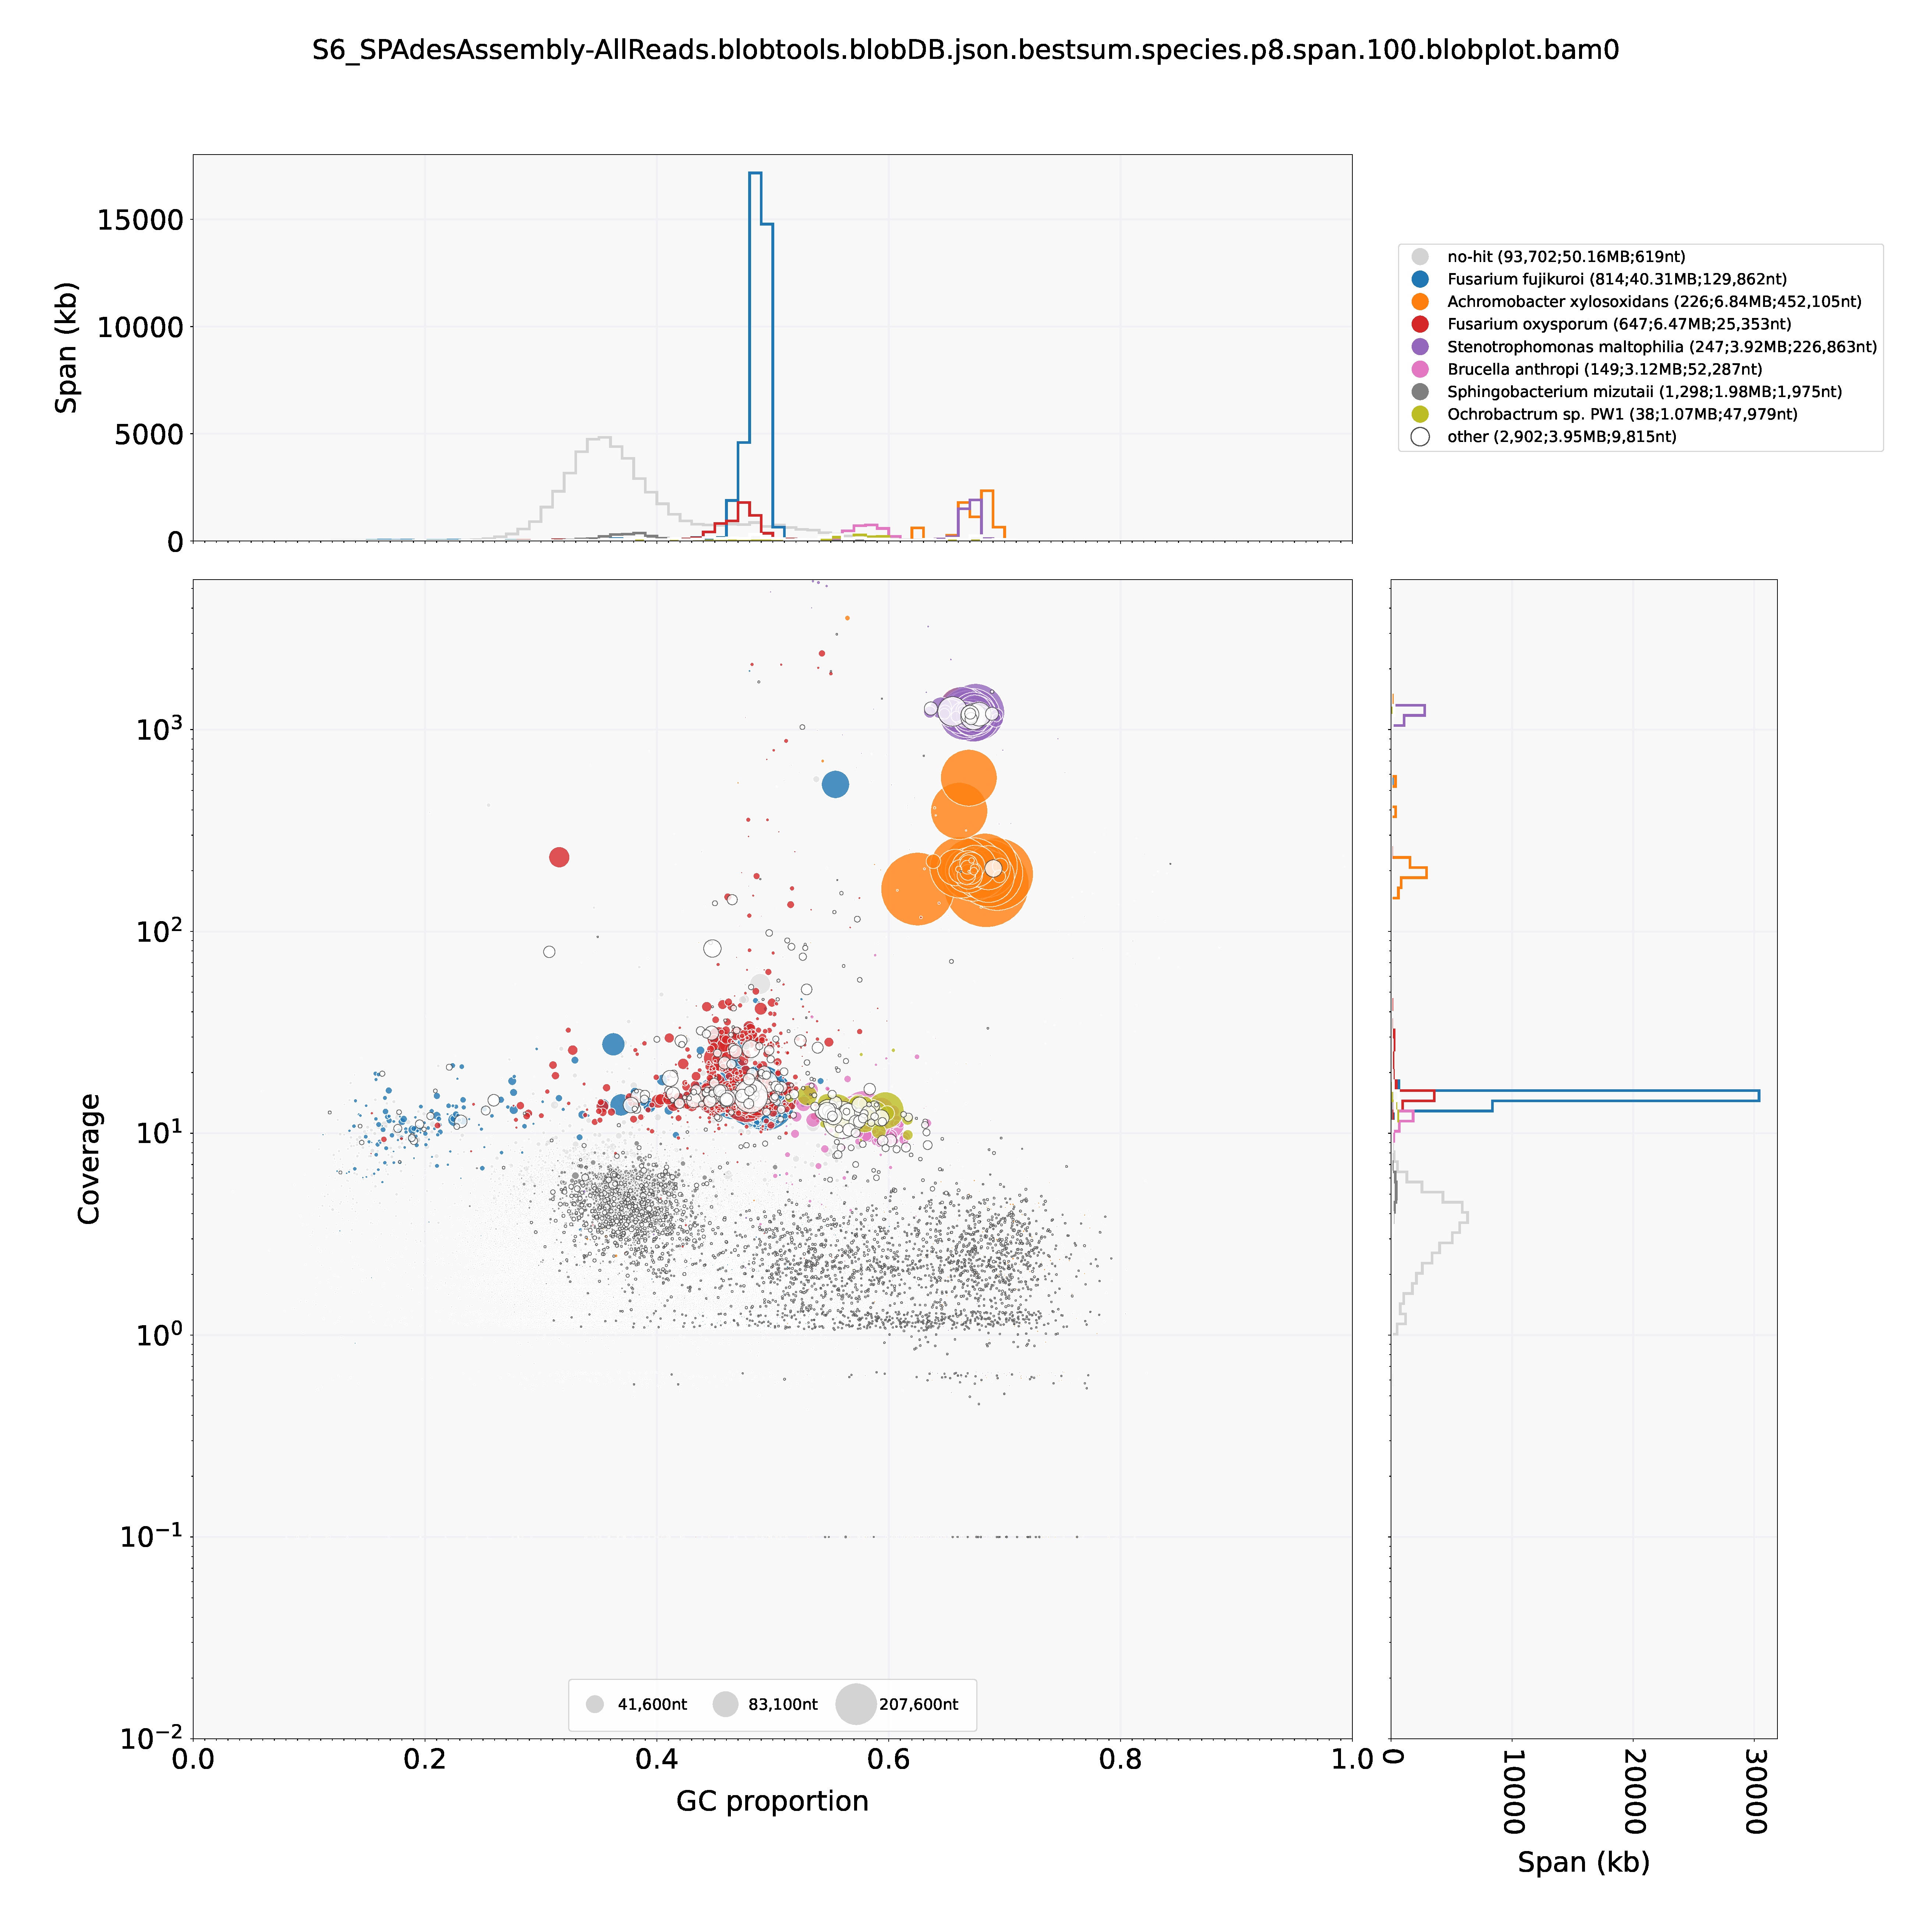
\includegraphics[width=\textwidth]{Appendices/S6_SPAdesAssembly-AllReads.blobtools.blobDB.json.bestsum.species.p8.span.100.blobplot.bam0.pdf}
        \caption{}
        \label{fig:BlobPlot-S6-All}
    \end{subfigure}
    \begin{subfigure}[]{0.9\textwidth}
        \centering
        \includegraphics[width=\textwidth]{Appendices/S6_SPAdesAssembly-AllReads.blobtools.blobDB.json.bestsum.species.p8.span.100.blobplot.read_cov.bam0.pdf}
        \caption{}
        \label{fig:BlobPlot_readcov-S6-All}
    \end{subfigure}
    \caption[BlobTools visualisations of the unfiltered S6 assembly]{\textbf{BlobTools visualisations of the unfiltered S6 assembly shows bacterial contamination.}
        \subref{fig:BlobPlot-S6-All} BlobPlot of S6. Sequences in the unfiltered assembly are depicted as circles, with diameter proportional to sequence length and coloured by taxonomic annotation based on BLASTN (v2.9.0+) of NCBI nt database.
        \subref{fig:BlobPlot_readcov-S6-All} Read coverage plot of the unfiltered S6 assembly. Mapped reads are shown by taxonomic group at the rank of species.}
        \label{fig:S6:BlobToolsAllreads}
\end{figure}
\bigskip

\begin{figure}[hp!]
    \centering
    \begin{subfigure}[]{0.9\textwidth}
        \centering
        \includegraphics[width=\textwidth]{Figures/TNAU_S32_AllContigs.blobtools.blobDB.json.bestsum.species.p8.span.100.blobplot.bam0.png}
        \caption{}
        \label{fig:BlobPlot-S32-All}
    \end{subfigure}
    \begin{subfigure}[]{0.9\textwidth}
        \centering
        \includegraphics[width=\textwidth]{Figures/TNAU_S32_AllContigs.blobtools.blobDB.json.bestsum.species.p8.span.100.blobplot.read_cov.bam0.png}
        \caption{}
        \label{fig:BlobPlot_readcov-S32-All}
    \end{subfigure}
    \caption[BlobTools visualisations of the unfiltered S32 assembly]{\textbf{BlobTools visualisations of the unfiltered S32 assembly shows bacterial contamination.}
        \subref{fig:BlobPlot-S32-All} BlobPlot of S32. Sequences in the unfiltered assembly are depicted as circles, with diameter proportional to sequence length and coloured by taxonomic annotation based on BLASTN (v2.9.0+) of NCBI nt database.
        \subref{fig:BlobPlot_readcov-S32-All} Read coverage plot of the unfiltered S32 assembly. Mapped reads are shown by taxonomic group at the rank of species.}
        \label{fig:S32:BlobToolsAllreads}
\end{figure}
\bigskip

\subsubsection{\acf{rbp2} Phylogeny of \textit{Fusarium} assemblies}

% Please add the following required packages to your document preamble:
% \usepackage{multirow}
% \usepackage{graphicx}
% \usepackage{lscape}
\begin{landscape}
\begin{table}[]
\centering
\captionsetup{width=\linewidth} 
\caption{[\Ac{tnau}\acf{tef} \acf{ncbi} and Fusariod-ID MSLT database searches.]\textbf{Best hits of extracted \acf{tef} sequences from the \acf{tnau} isolate \textit{de novo} assemblies against the Fusariod-ID MSLT database and \ac{ncbi}}}
\label{tab:Tef1-MLSTdb}
\resizebox{\columnwidth}{!}{%
\begin{tabular}{cccc}
\multirow{2}{*}{\textbf{TNAU Isolate Assembly}} & \multicolumn{3}{c}{\textbf{Fusariod-ID MSLT database}}                                     \\ \cline{2-4} 
                                                & Match 1                      & Match 2                      & Match 3                      \\ \hline
\textbf{S6 All reads}                           & \textit{F. oxysporum} Species Complex & \textit{F. oxysporum} Species Complex & \textit{F. oxysporum} Species Complex \\
\textbf{S6 \textit{F. oxysporum}  Reads}                 & \textit{F. oxysporum} Species Complex & \textit{F. oxysporum} Species Complex & \textit{F. oxysporum} Species Complex \\
\textbf{S16}                                    & \textit{F. oxysporum} Species Complex  & \textit{F. oxysporum} Species Complex  & \textit{F. oxysporum} Species Complex  \\
\textbf{S32 All reads}                          & No Matches                   & No Matches                   & No Matches                   \\
\textbf{S32 \textit{F. oxysporum}  Reads}                & No Matches                   & No Matches                   & No Matches                   \\
\textbf{S32 \textit{F. oxysporum}}                        & No Matches                   & No Matches                   & No Matches                  
\end{tabular}%
}
\end{table}
\end{landscape}

\begin{figure}[htp!]
    \centering
    \includegraphics[width=14cm]{Appendices/RPNii-Phylogeny.pdf}
    \caption[\Acl{rbp2} phylogeny of \acl{tnau} \textit{Fusarium} isolates.]{\textbf{\Acl{rbp2} phylogeny of \acl{tnau} \textit{Fusarium} isolates.} \Ac{tnau} isolates S16, S32 and SY-2 sit within the \acf{FFSC} clade. The isolates from \ac{tnau} are shown in red text. The \acf{Fs} clade is shown in pink. \Acf{Focub4} isolates are in blue. \Acf{Focub1} isolates are shown in green. \acf{Focub} isolates with race not recorded are shown in yellow. Percentages represent values from 1000 bootstrap replicates. The tree is rooted through \textit{Fusarium graminearum} PH-1 \ac{rbp2}.}
    \label{fig:rbp2Phylo}
\end{figure}
\bigskip

\end{document}                       %% Done.

